\subsection{Thiết kế giao diện hệ thống}

Trong phần này, toàn bộ giao diện màn hình của hệ thống được tổ chức và trình bày chi tiết theo 4 phân hệ người dùng chính (Customer, Staff, Branch Admin, Admin) và giao diện xác thực chung. Việc thiết kế tuân thủ nguyên tắc lấy người dùng làm trung tâm, phân chia luồng thao tác rõ ràng nhằm đảm bảo hiệu suất vận hành và trải nghiệm liền mạch.

\providecommand{\FloatBarrier}{\relax}

\subsubsection{Giao diện xác thực chung}

Giao diện đăng nhập là điểm tiếp xúc đầu tiên và cũng là chốt chặn bảo mật quan trọng nhất của hệ thống. Dựa trên thông tin định danh được cung cấp, hệ thống sẽ xác thực và tự động điều hướng người dùng đến đúng phân hệ tương ứng với vai trò và quyền hạn của họ.

\begin{figure}[H]
    \centering
    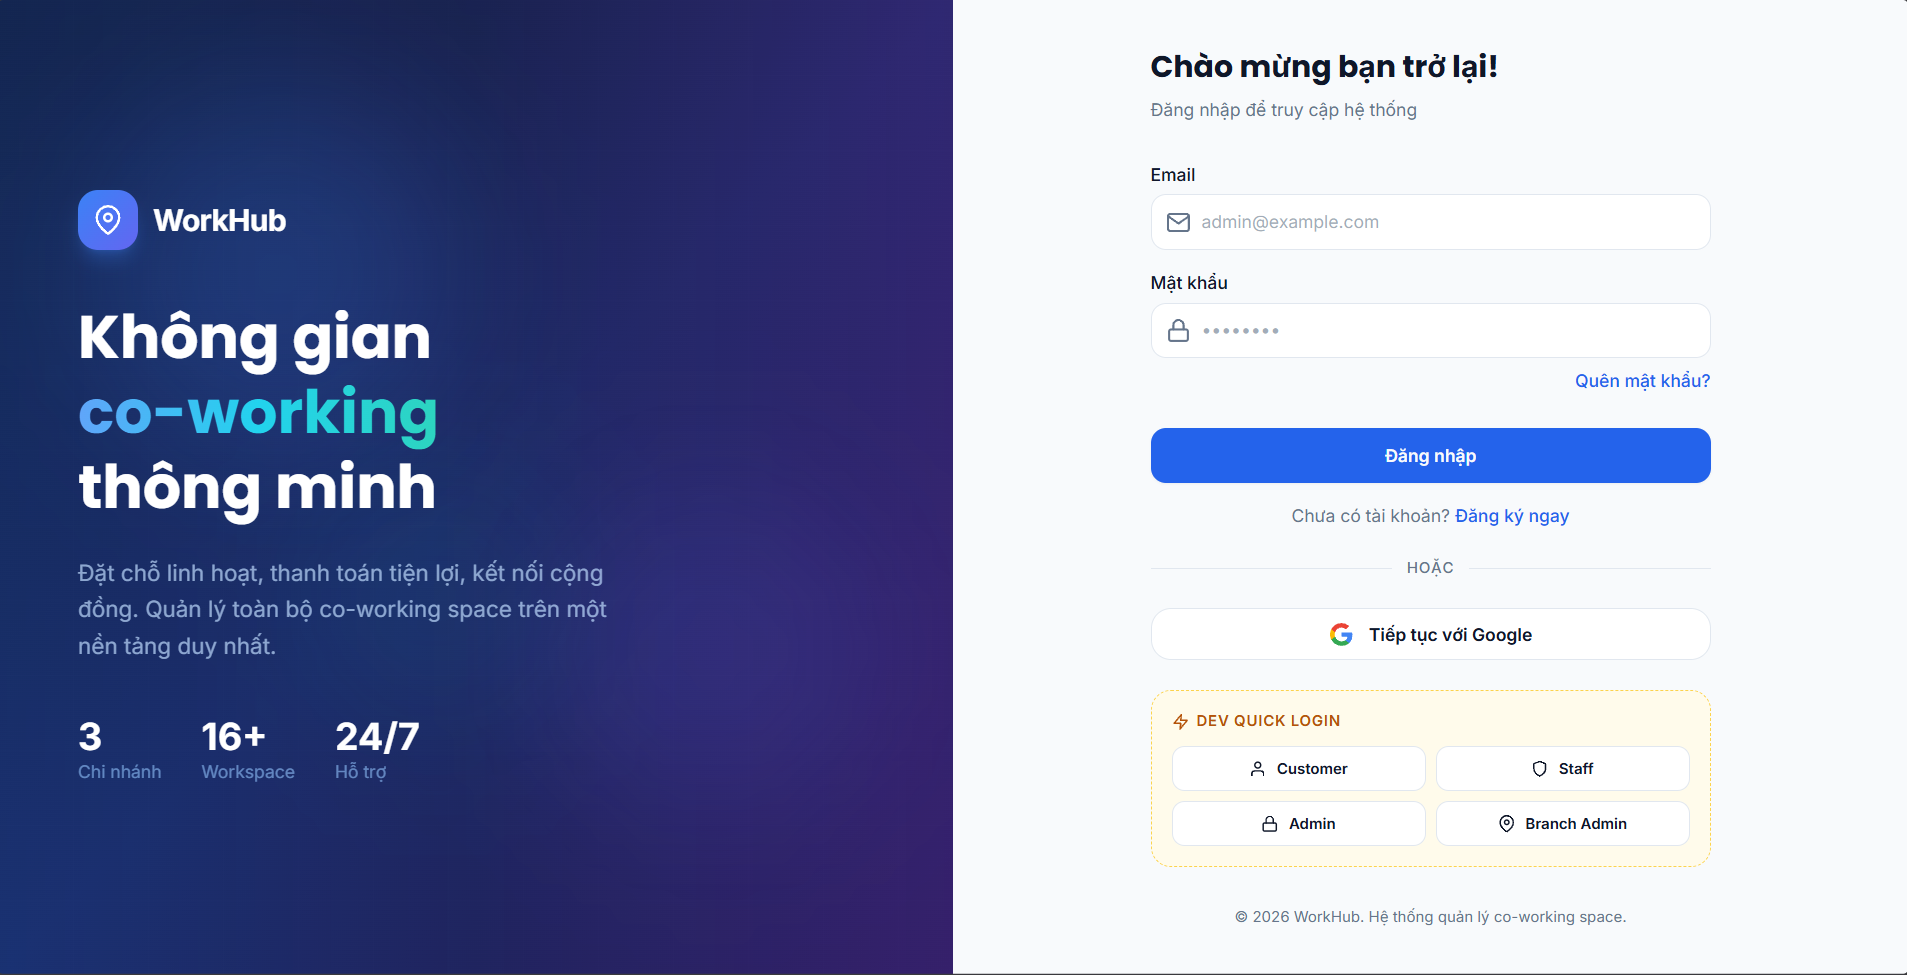
\includegraphics[width=0.9\textwidth]{Images/Chuong4/login_page.png}
    \caption{Giao diện xác thực định danh và phân luồng người dùng}
    \label{fig:ui_login_page}
\end{figure}

\FloatBarrier
\newpage

\subsubsection{Phân hệ Giao diện Khách hàng (Customer)}

Phân hệ khách hàng cung cấp các công cụ trực quan giúp người dùng cuối dễ dàng tiếp cận không gian, quản lý quá trình sử dụng dịch vụ và mở rộng các mối quan hệ chuyên môn.

Giao diện Đặt chỗ đóng vai trò như một danh mục điện tử thông minh, cho phép người dùng tìm kiếm, lọc và tra cứu thông tin về các vị trí làm việc, phòng họp dựa trên nhiều tiêu chí như chi nhánh, sức chứa và mức giá.

\begin{figure}[H]
    \centering
    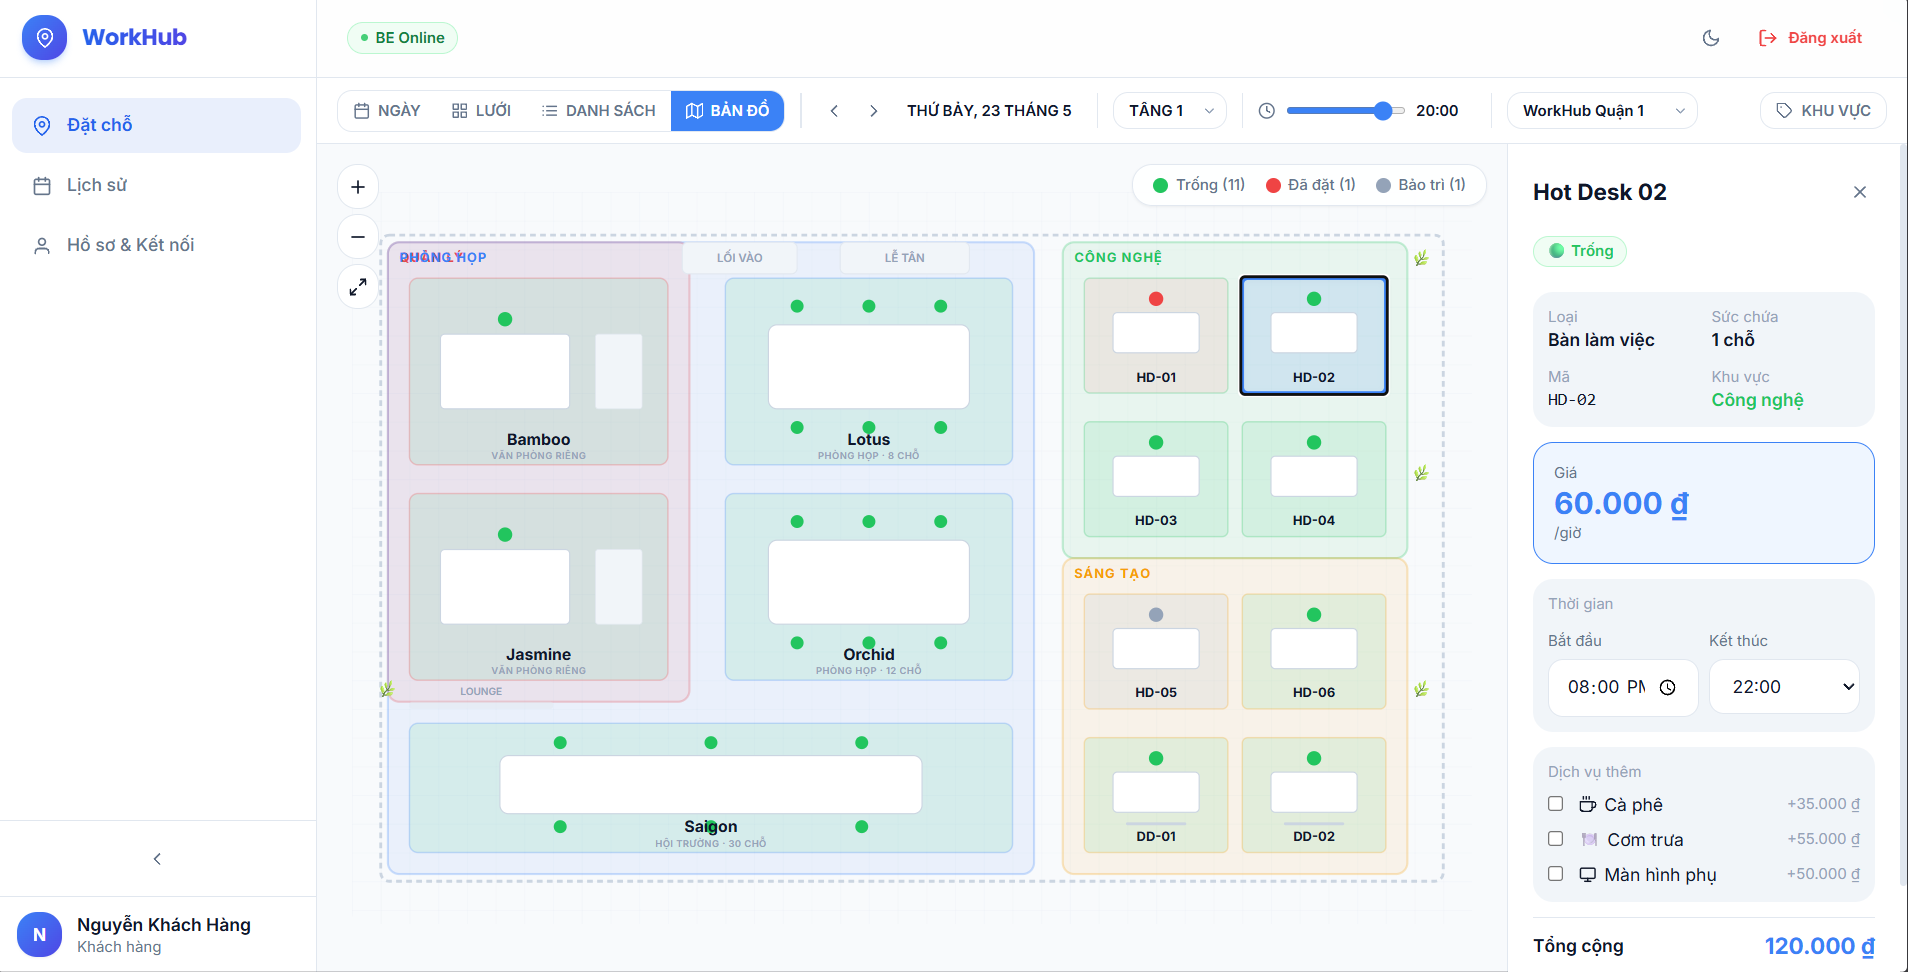
\includegraphics[width=0.9\textwidth]{Images/Chuong4/customer-booking-page.png}
    \caption{Giao diện tìm kiếm và đặt chỗ}
    \label{fig:ui_booking_page}
\end{figure}
\FloatBarrier

Giao diện Thanh toán cung cấp tính minh bạch về mặt tài chính. Mọi giao dịch phát sinh từ việc đặt chỗ, mua thêm dịch vụ hay phí phạt đều được liệt kê chi tiết, giúp khách hàng dễ dàng đối soát chi tiêu.

\begin{figure}[H]
    \centering
    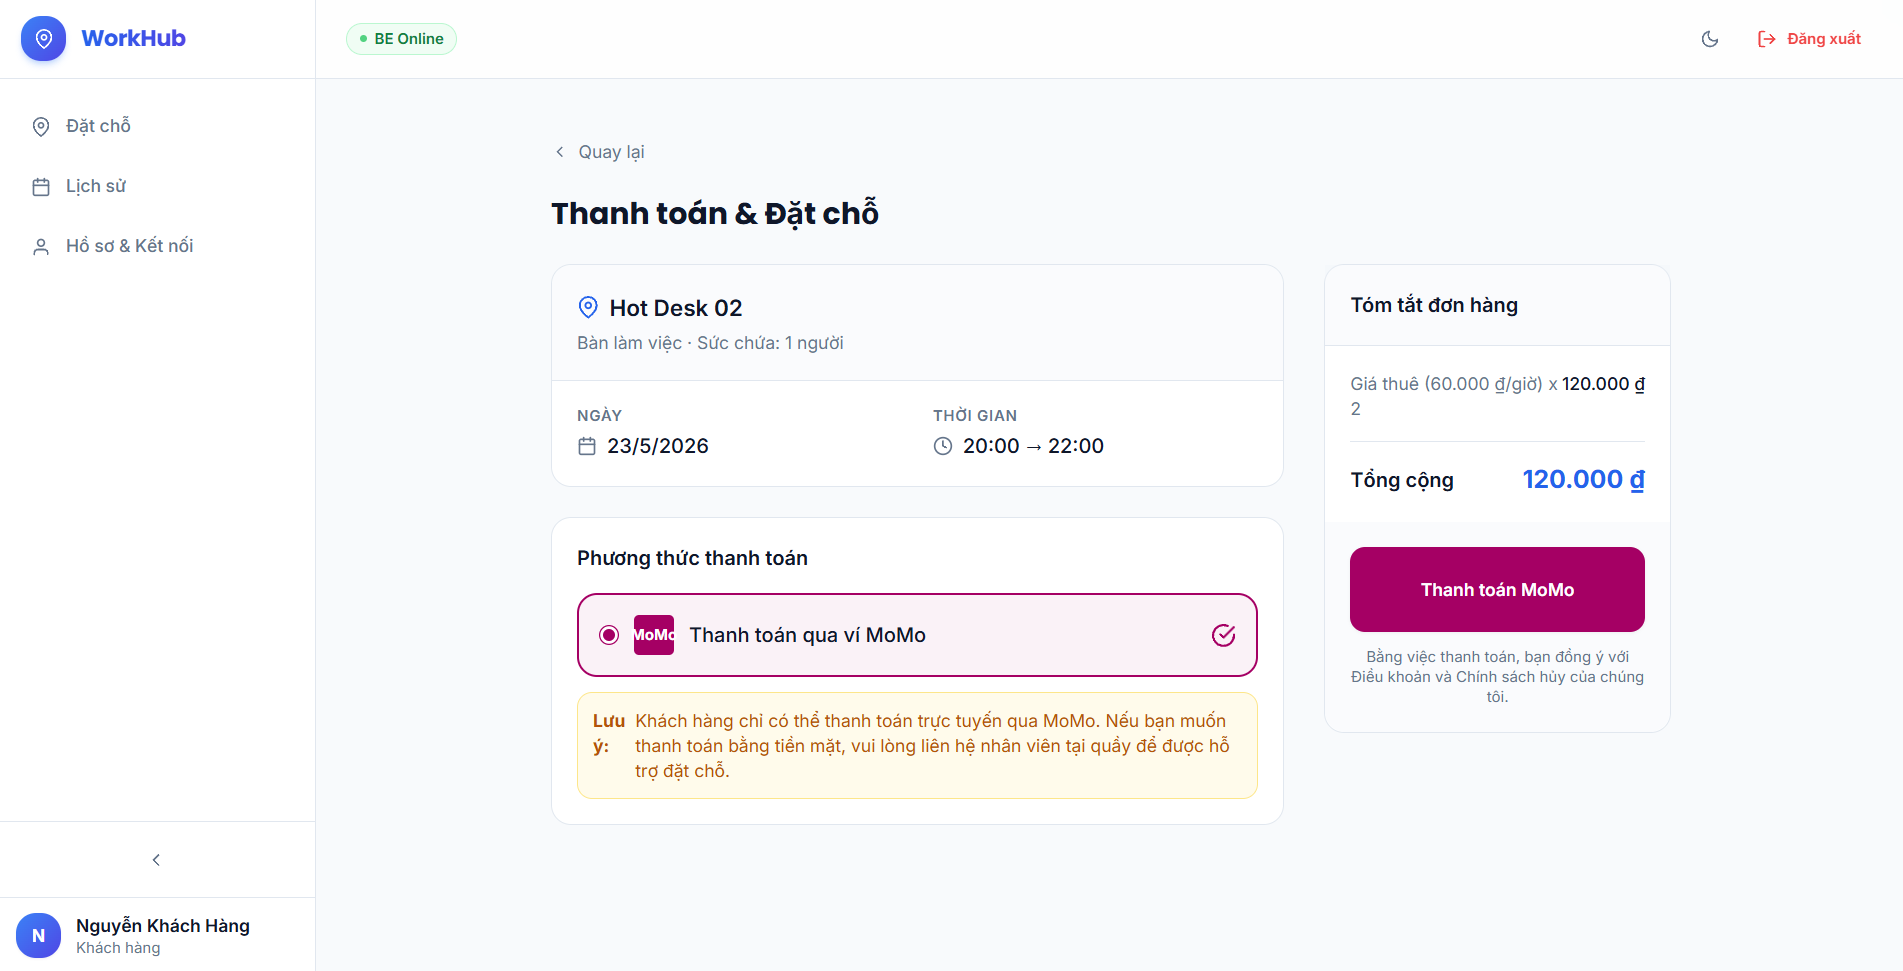
\includegraphics[width=0.9\textwidth]{Images/Chuong4/customer-payment-page.png}
    \caption{Giao diện thanh toán của khách hàng}
    \label{fig:ui_payment_page}
\end{figure}

\FloatBarrier

Giao diện Lịch sử đặt chỗ cá nhân là nơi tổng hợp toàn bộ lịch trình của người dùng. Tại đây, khách hàng có thể theo dõi lịch sử sử dụng trong quá khứ và chủ động thực hiện các thao tác thay đổi hoặc hủy lịch khi cần thiết.

\begin{figure}[H]
    \centering
    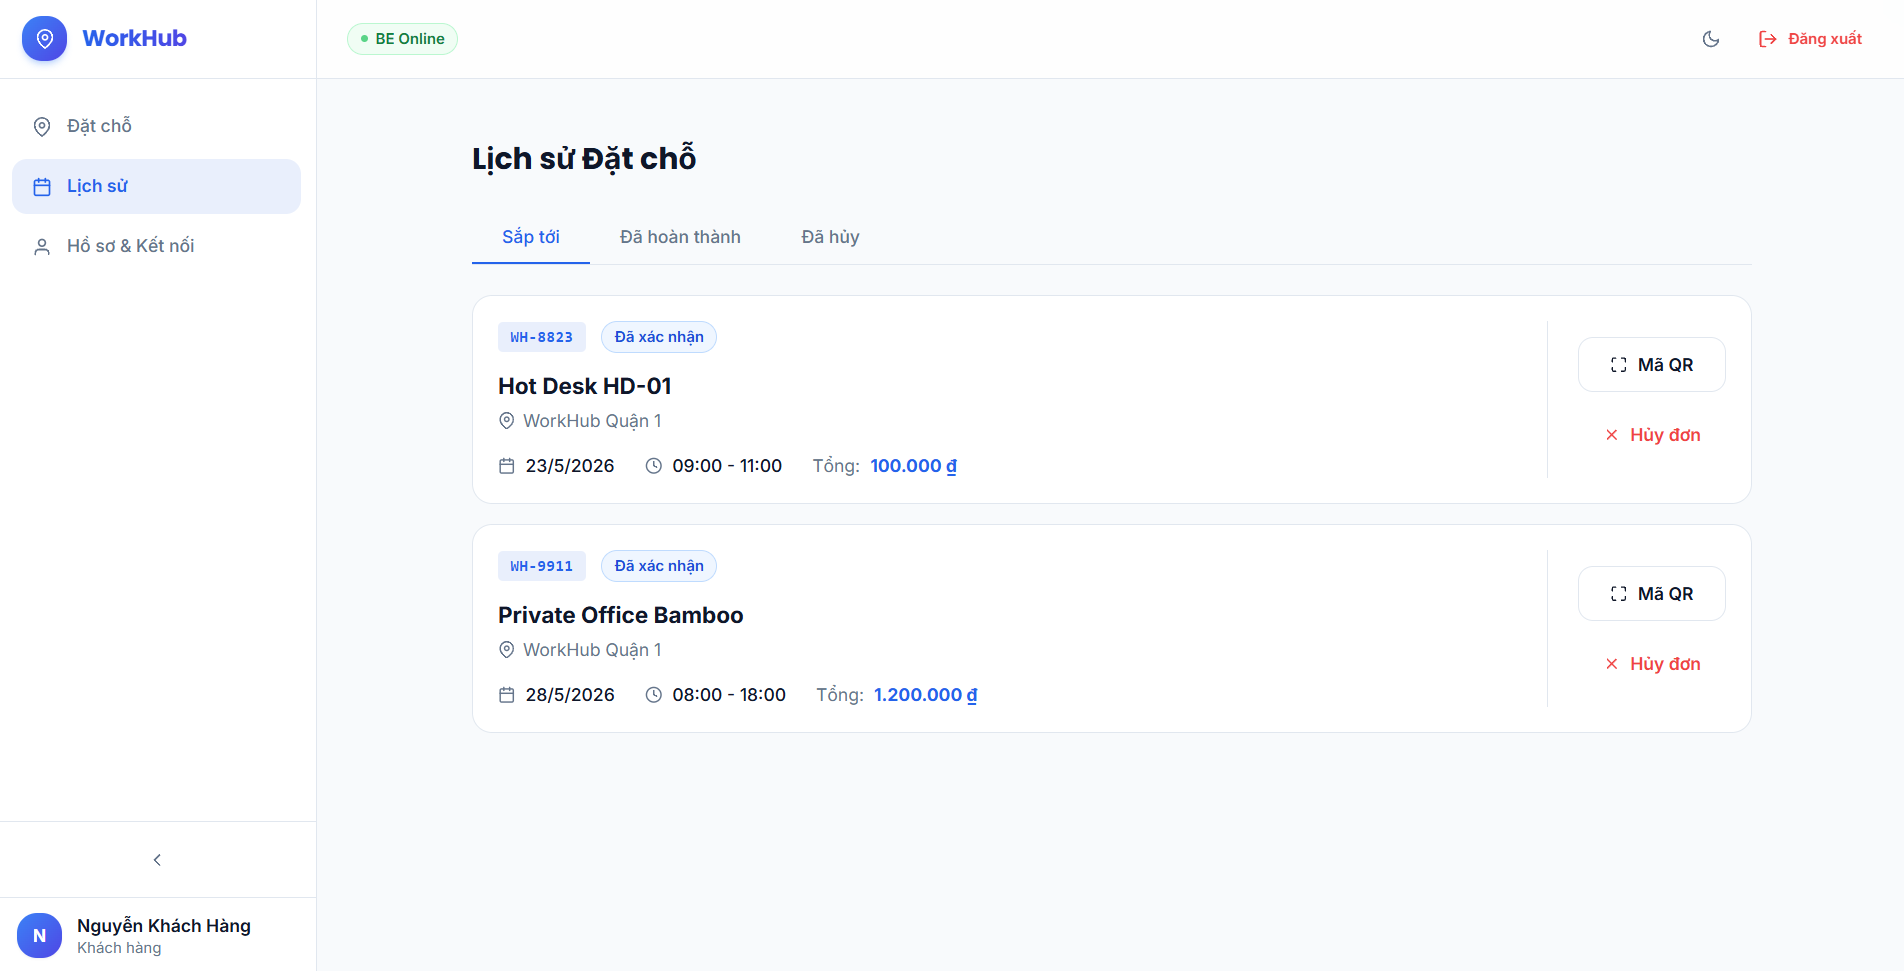
\includegraphics[width=0.9\textwidth]{Images/Chuong4/customer-history-page.png}
    \caption{Giao diện thống kê lịch sử sử dụng dịch vụ}
    \label{fig:ui_my_bookings_page}
\end{figure}

\begin{figure}[H]
    \centering
    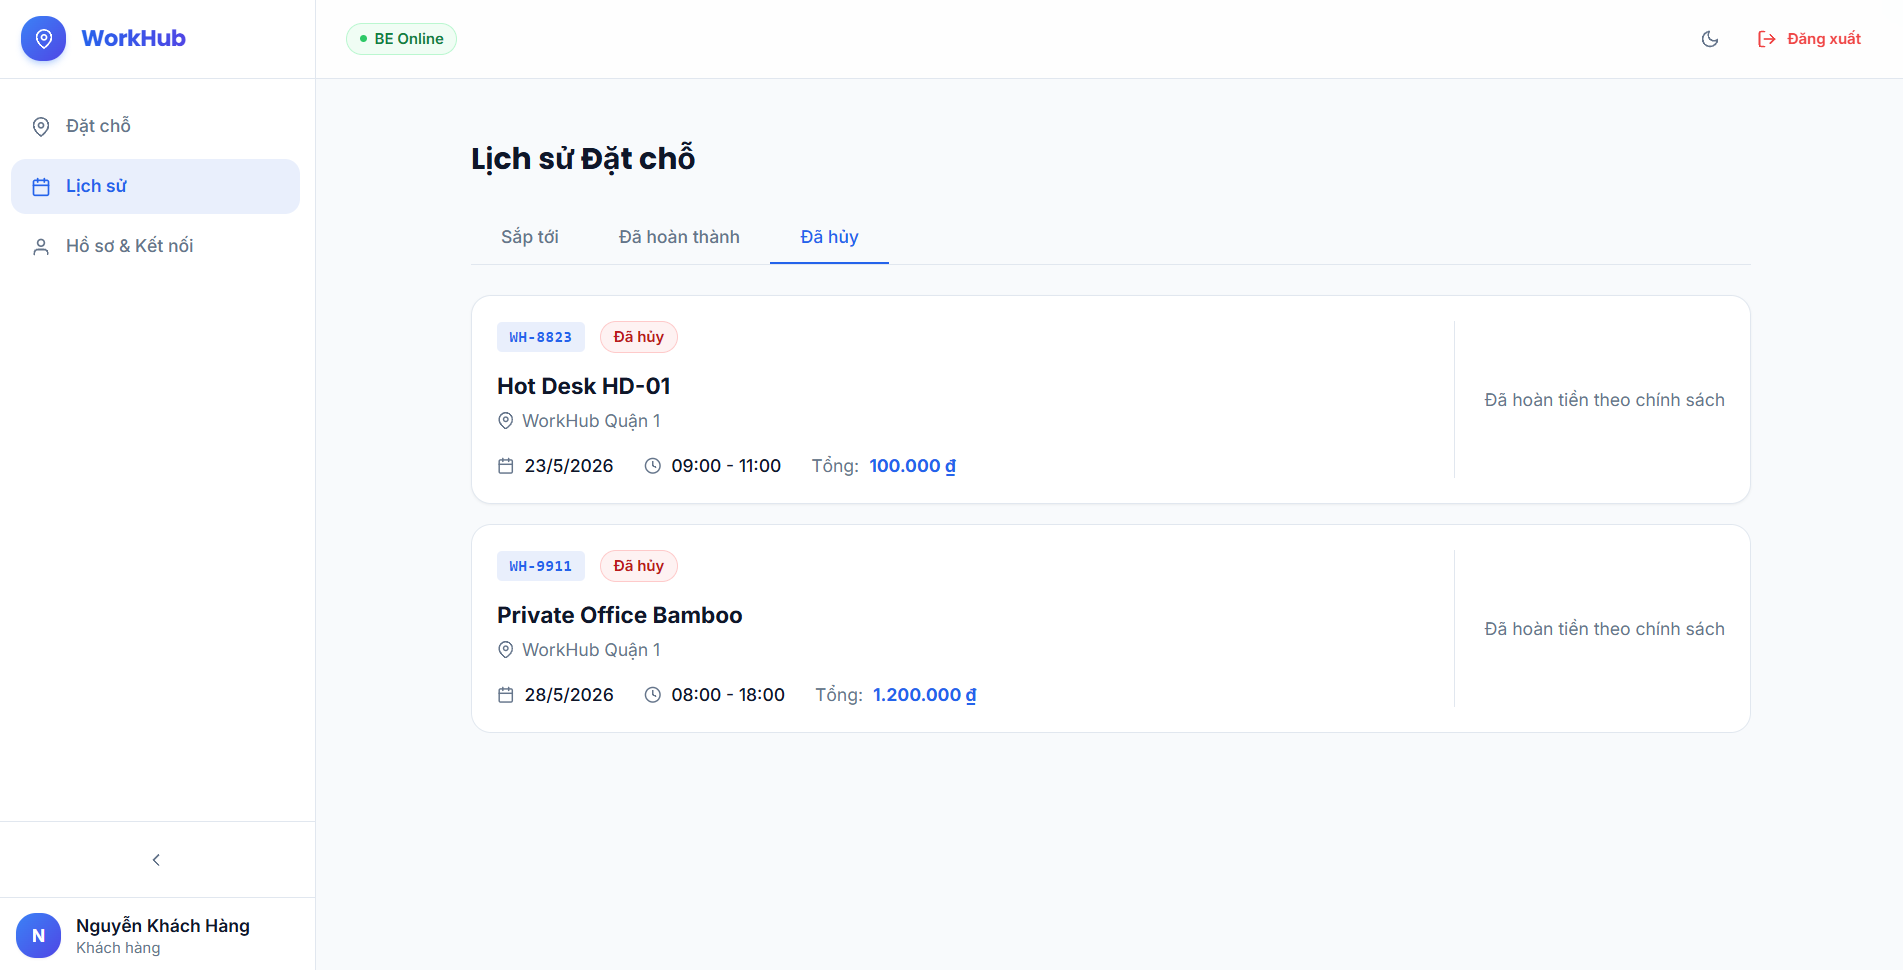
\includegraphics[width=0.9\textwidth]{Images/Chuong4/customer-cancel-page.png}
    \caption{Giao diện lịch sử hủy}
    \label{fig:ui_cancel_page}
\end{figure}
\FloatBarrier
\newpage

Giao diện Chỉnh sửa hồ sơ giúp người dùng thay đổi tùy chỉnh thông tin cơ bản, thông tin liên hệ hay kỹ năng và sở thích. Tính năng này giúp người dùng tùy chỉnh hồ sơ để có thể kết nối với cộng đồng.

\begin{figure}[H]
    \centering
    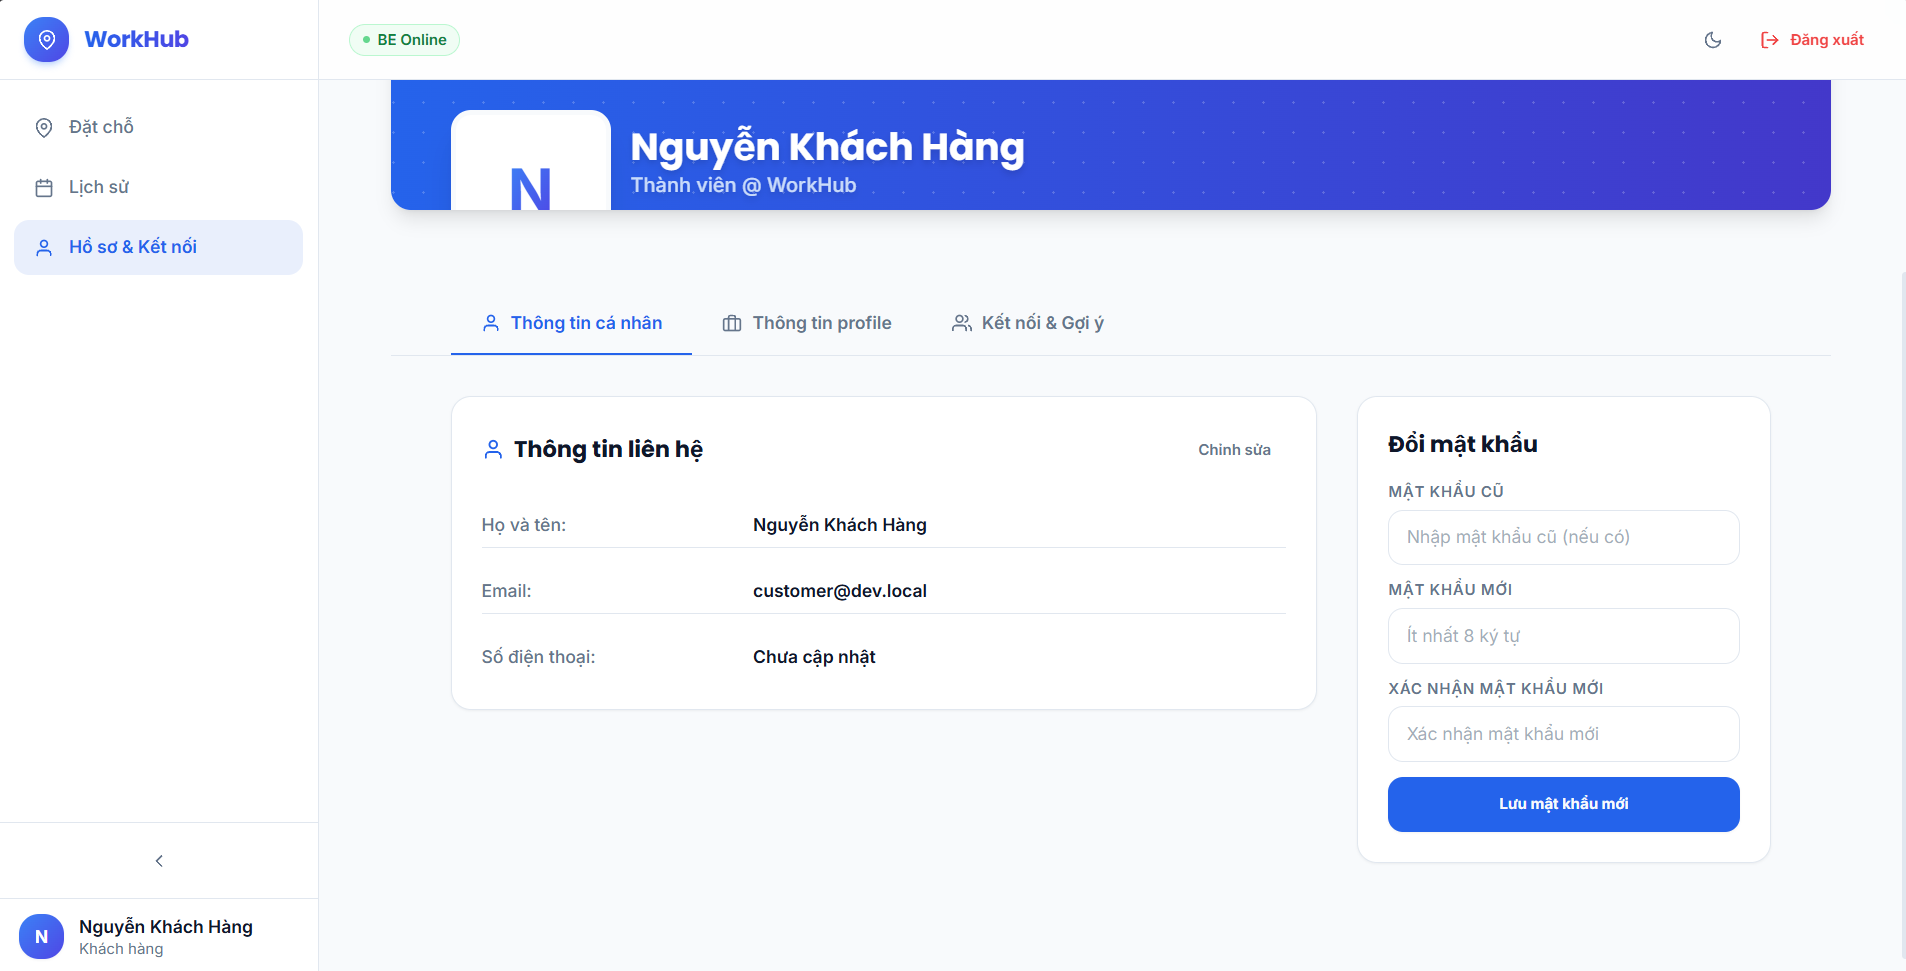
\includegraphics[width=0.9\textwidth]{Images/Chuong4/customer-profile-page.png}
    \caption{Giao diện chỉnh sửa thông tin hồ sơ người dùng}
    \label{fig:ui_profile_page}
\end{figure}
\FloatBarrier
\newpage

Giao diện Gợi ý kết nối đối tác ứng dụng thuật toán so khớp hồ sơ năng lực nhằm đề xuất những cá nhân có chuyên môn phù hợp trong cùng mạng lưới. Tính năng này nâng cao giá trị gia tăng cho người dùng thông qua việc thúc đẩy cơ hội hợp tác và chia sẻ kinh nghiệm.

\begin{figure}[H]
    \centering
    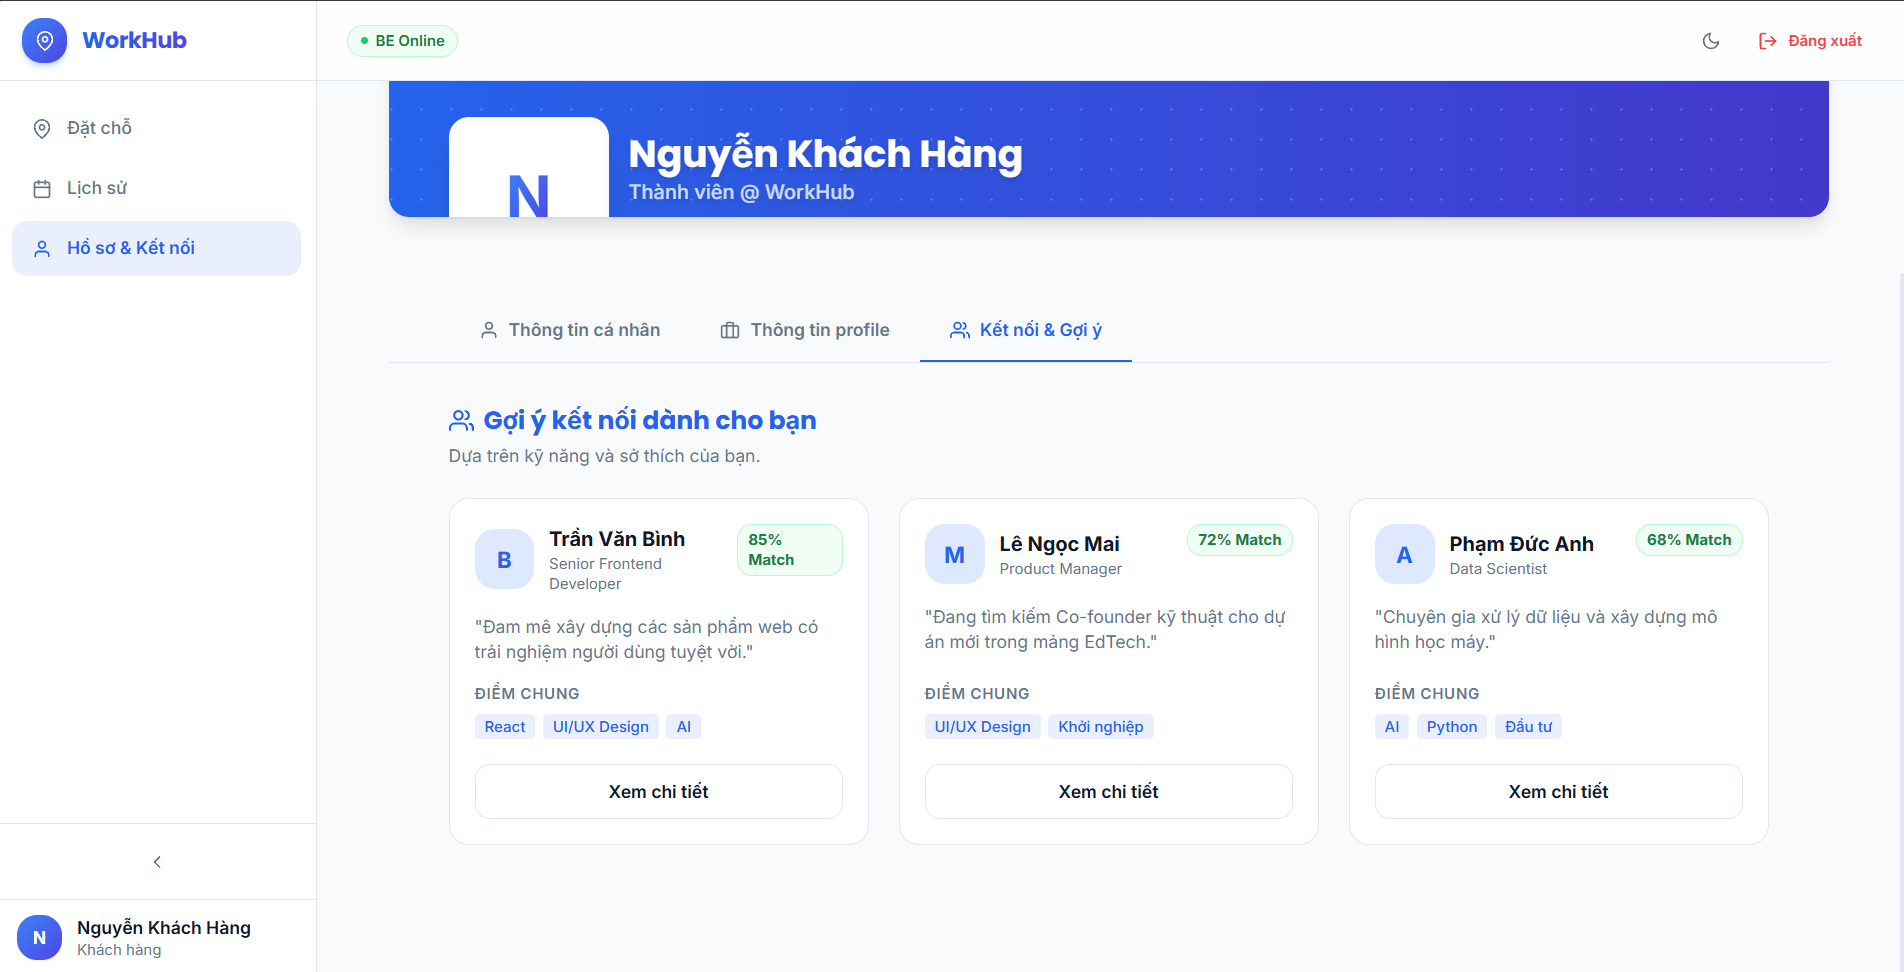
\includegraphics[width=0.9\textwidth]{Images/Chuong4/customer-connect-page.png}
    \caption{Giao diện gợi ý và hỗ trợ tương tác trong hệ sinh thái}
    \label{fig:ui_partner_match_page}
\end{figure}



\FloatBarrier
\newpage

\subsubsection{Phân hệ Giao diện Nhân viên vận hành (Staff)}

Nhóm giao diện dành cho nhân viên được thiết kế nhằm mục đích hỗ trợ công tác trực tại quầy, quản lý không gian vật lý và xử lý nhanh chóng các nghiệp vụ phát sinh hàng ngày.

Bảng điều khiển hoạt động cung cấp cái nhìn tổng quan theo thời gian thực về tình trạng lấp đầy của toàn chi nhánh, giúp nhân viên nhận diện nhanh các vị trí đang trống, khu vực quá tải và theo dõi lưu lượng khách hiện tại.

\begin{figure}[H]
    \centering
    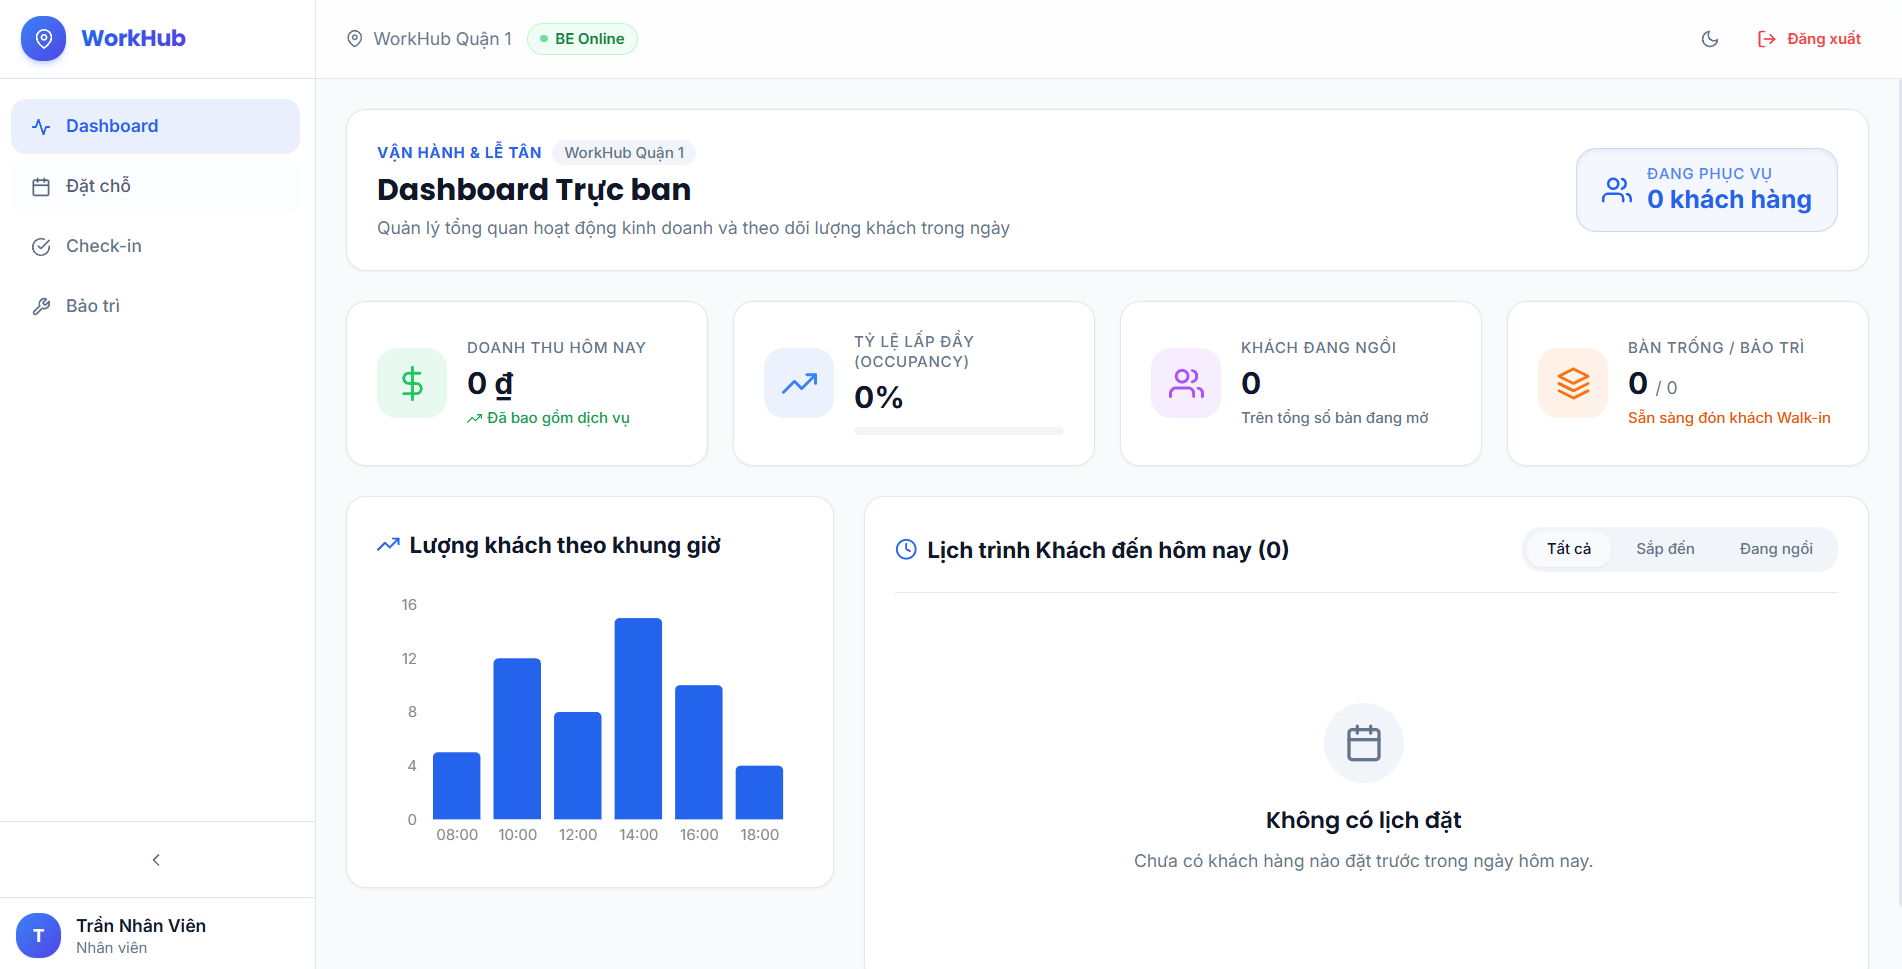
\includegraphics[width=0.9\textwidth]{Images/Chuong4/staff-dashboard.png}
    \caption{Giao diện Dashboard theo thời gian thực}
    \label{fig:ui_staff_dashboard_page}
\end{figure}

\FloatBarrier

\newpage

Đối với khách hàng chưa đặt trước qua nền tảng, giao diện Đặt chỗ trực tiếp cung cấp quy trình khởi tạo đơn vị dịch vụ nhanh chóng, cho phép nhân viên chọn loại không gian, cập nhật dịch vụ đi kèm và hoàn tất thao tác chỉ trong vài bước cơ bản.

\begin{figure}[H]
    \centering
    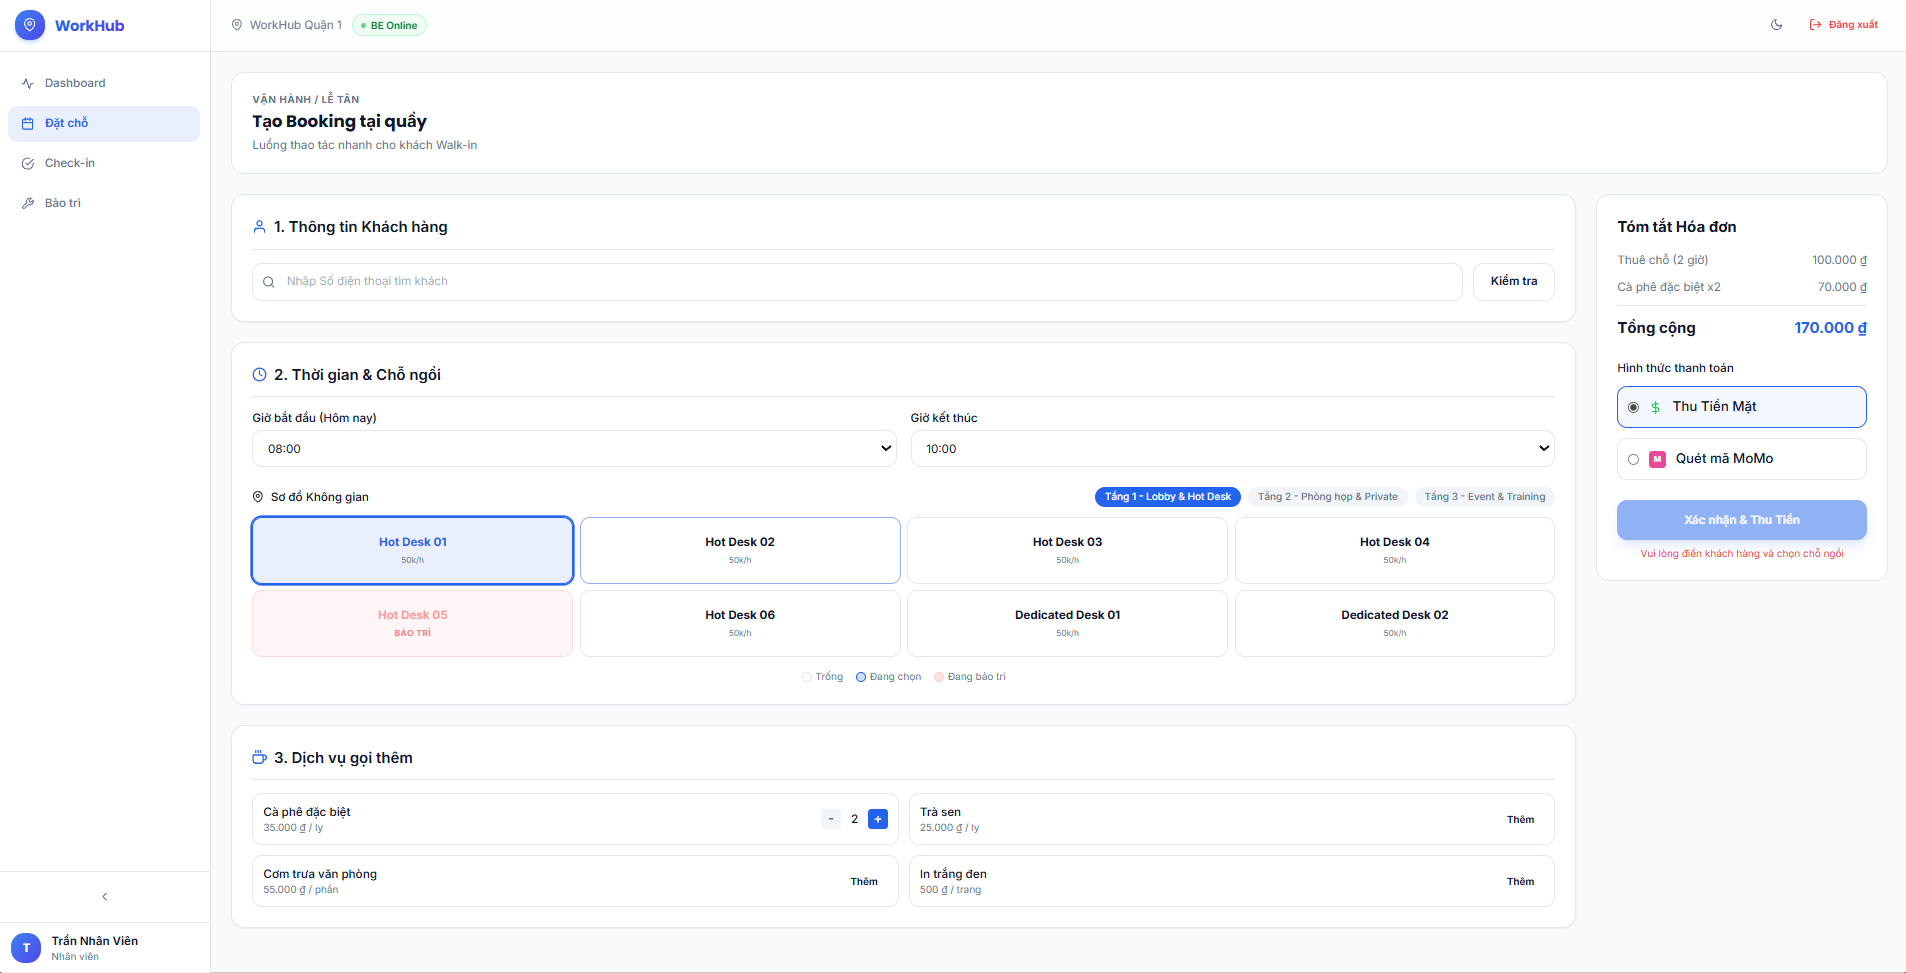
\includegraphics[width=0.9\textwidth]{Images/Chuong4/staff-booking.png}
    \caption{Giao diện hỗ trợ khởi tạo booking cho khách tại quầy}
    \label{fig:ui_staff_booking_page}
\end{figure}

\FloatBarrier
Giao diện Check-in được thiết kế tối giản quy trình xác thực. Nhân viên sử dụng giao diện này để ghi nhận thời điểm khách hàng bắt đầu hoặc kết thúc ca sử dụng, đảm bảo tính chính xác cho dữ liệu hệ thống.

\begin{figure}[H]
    \centering
    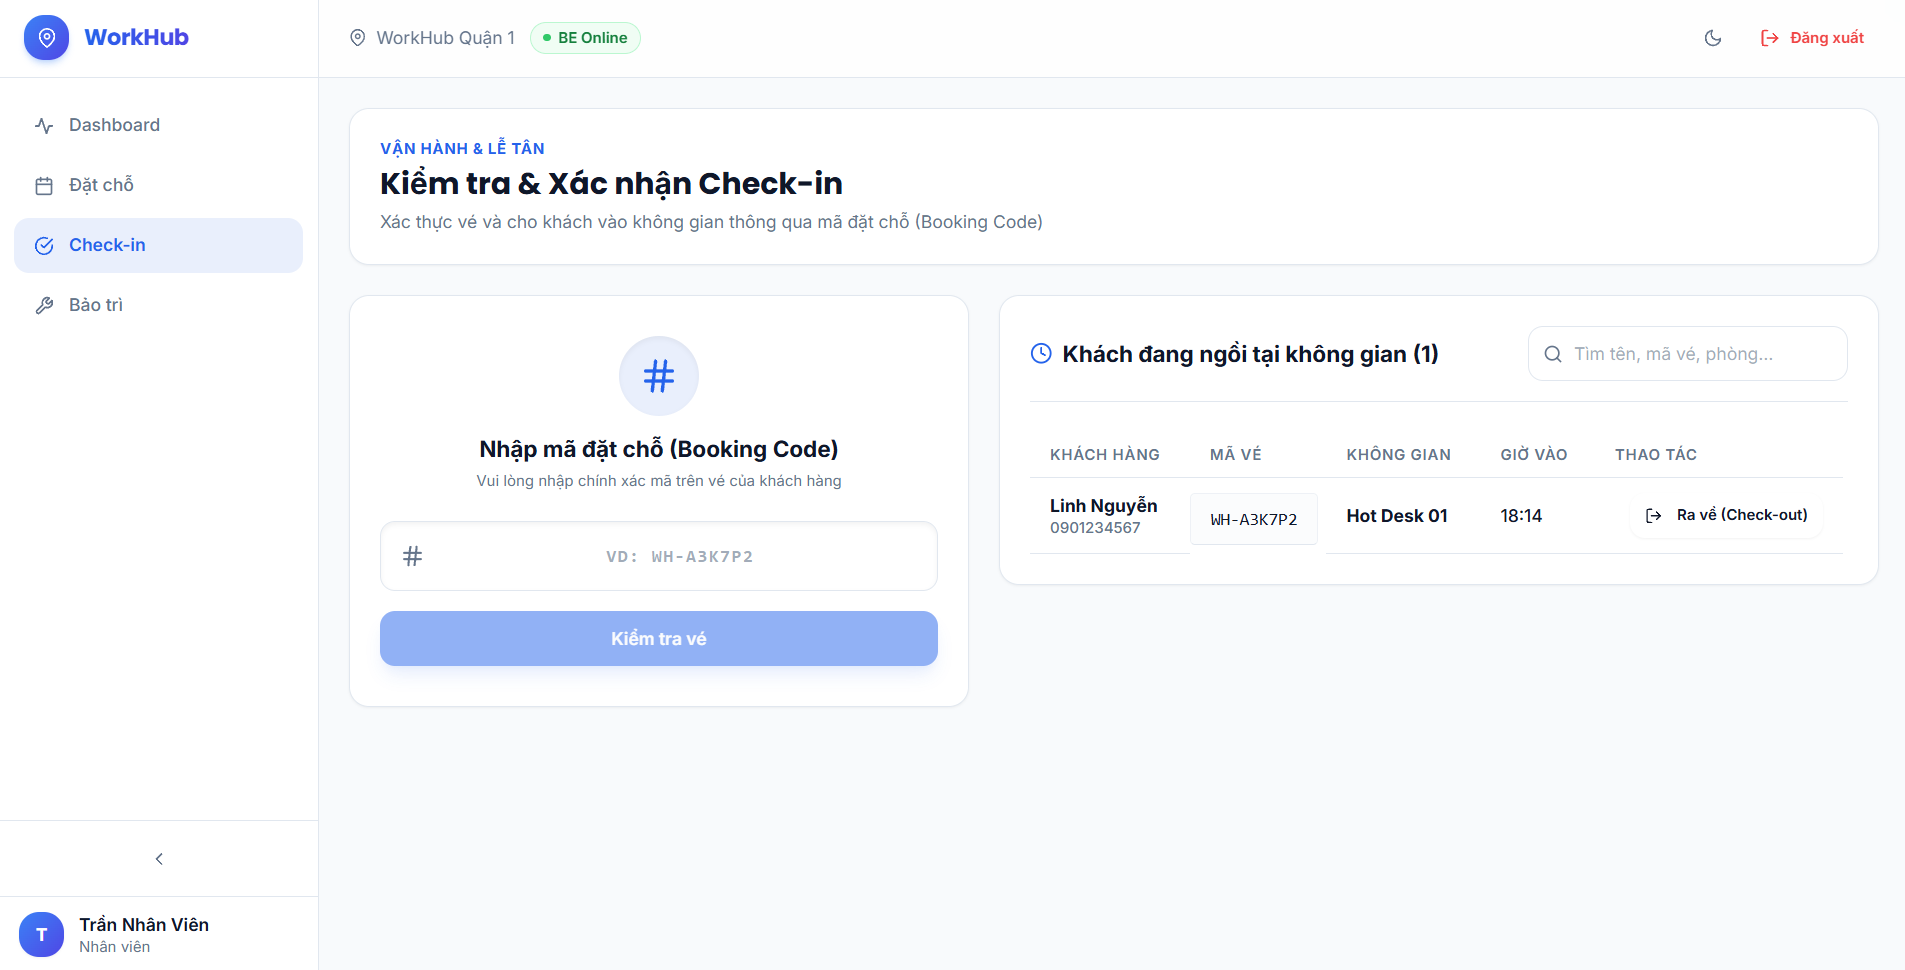
\includegraphics[width=0.9\textwidth]{Images/Chuong4/staff-check.png}
    \caption{Giao diện checkin và checkout tại quầy}
    \label{fig:ui_staff_check_page}
\end{figure}

\FloatBarrier
\newpage

Để đảm bảo chất lượng cơ sở vật chất, giao diện Quản lý bảo trì cho phép nhân viên ghi nhận các sự cố hỏng hóc, thiết lập khu vực ngừng hoạt động tạm thời và theo dõi tiến độ sửa chữa để không ảnh hưởng đến trải nghiệm khách hàng.

\begin{figure}[H]
    \centering
    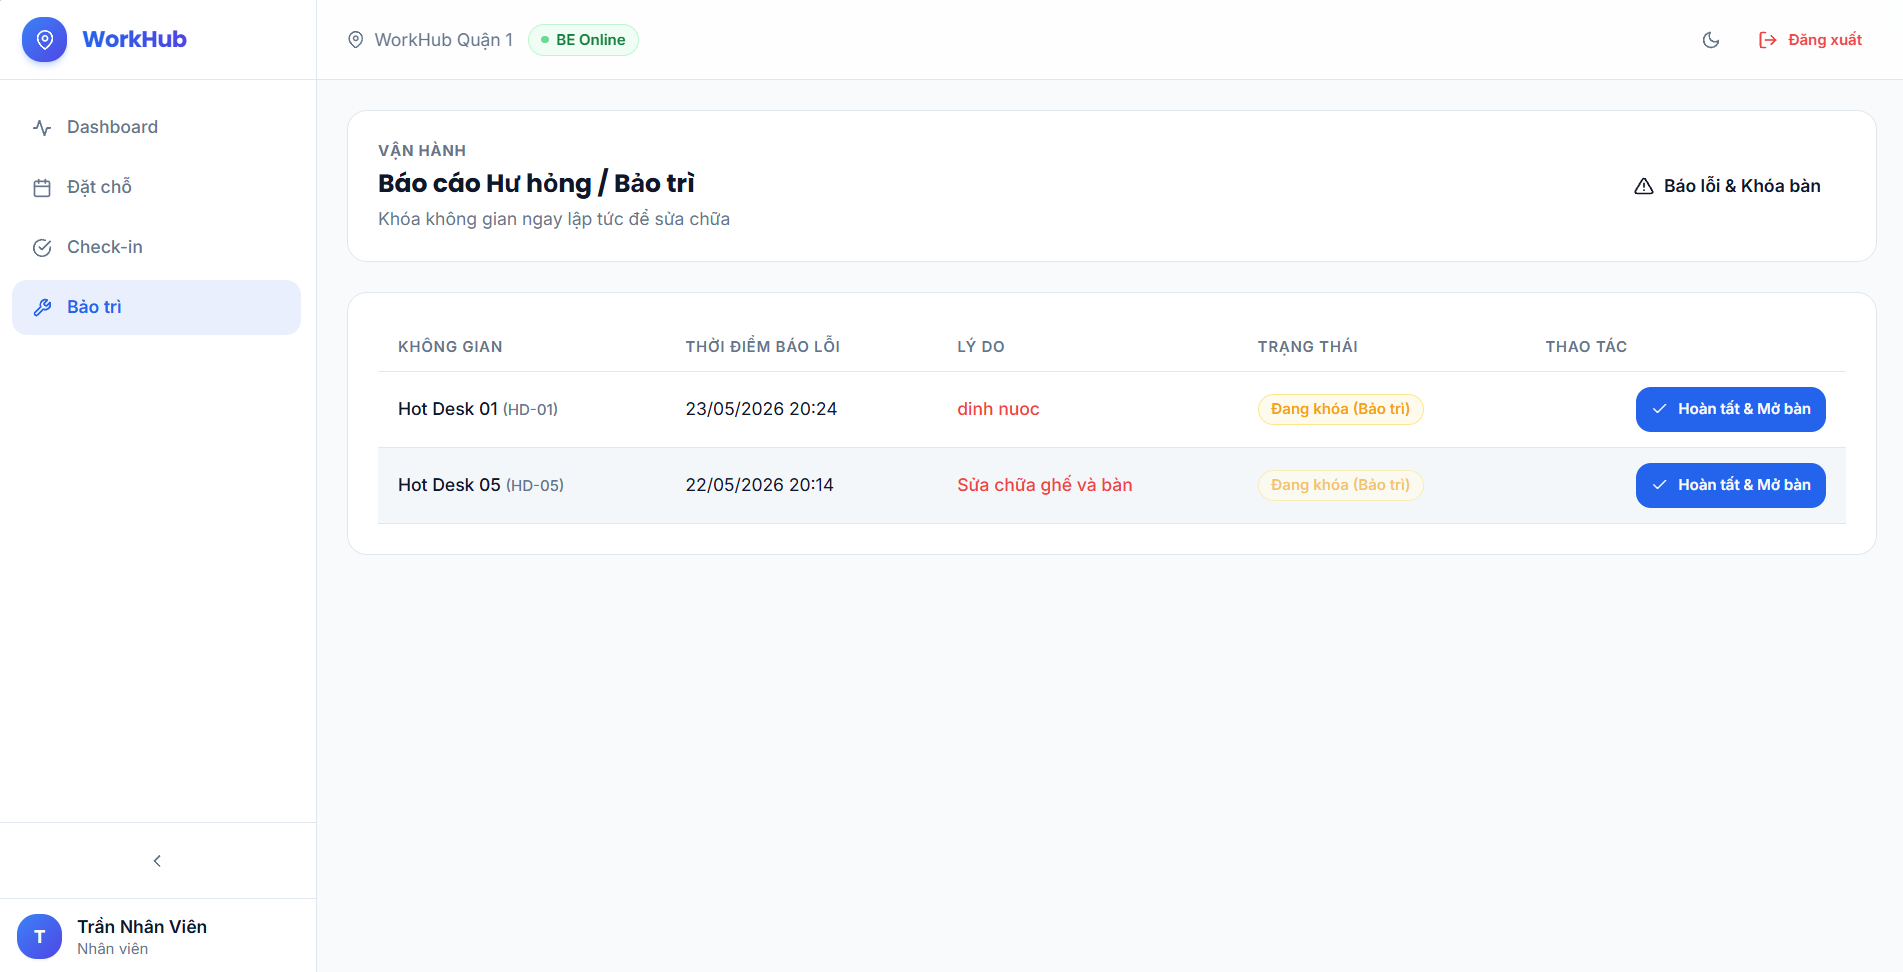
\includegraphics[width=0.9\textwidth]{Images/Chuong4/staff-maintenance.png}
    \caption{Giao diện báo cáo sự cố và theo dõi tiến độ bảo trì cơ sở vật chất}
    \label{fig:ui_maintenance_page}
\end{figure}

\FloatBarrier

\subsubsection{Phân hệ Giao diện Quản lý chi nhánh (Branch Admin)}

Cấp quản lý chi nhánh được cung cấp bộ công cụ chuyên sâu để tự chủ vận hành, quản trị nguồn lực và tối ưu hóa doanh thu tại cơ sở do mình phụ trách.

Giao diện Quản lý không gian cho phép cấu hình sơ đồ tầng, định vị các khu vực chức năng và thiết lập sức chứa tối đa. Các thông số này là cơ sở dữ liệu quan trọng để hệ thống tính toán khả năng phục vụ.

\begin{figure}[H]
    \centering
    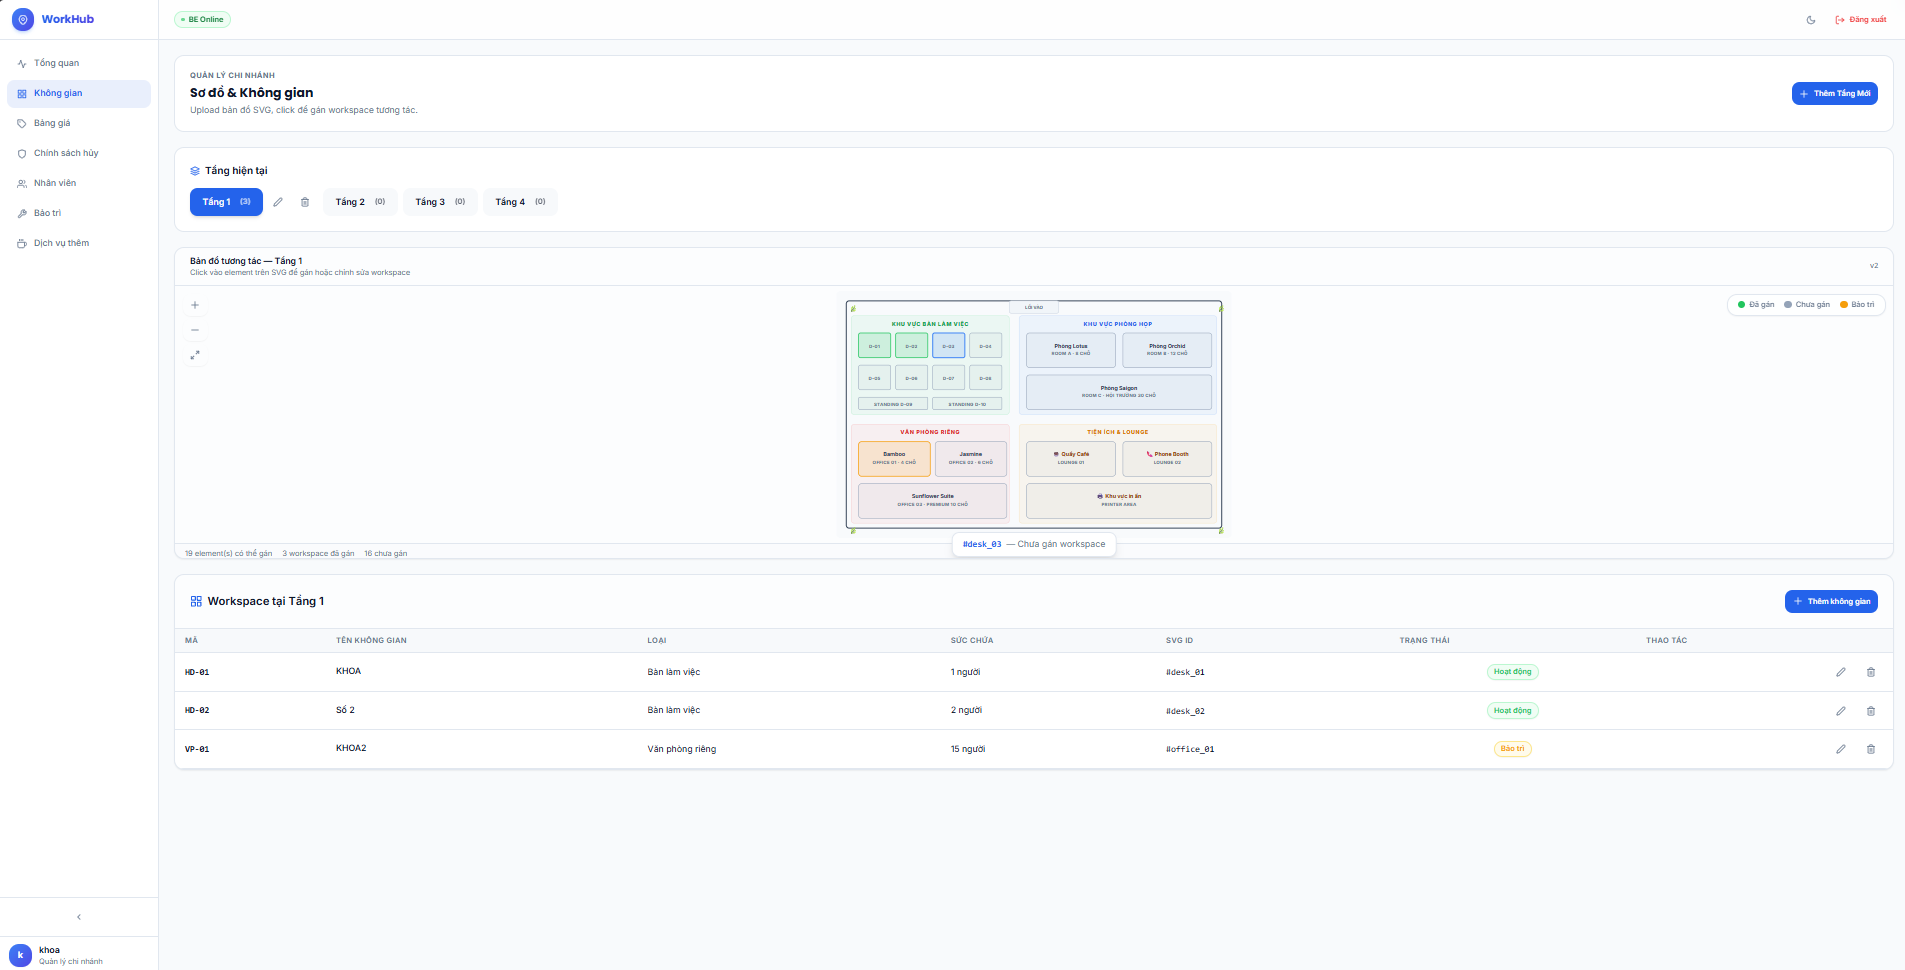
\includegraphics[width=0.9\textwidth]{Images/Chuong4/ui_ba_workspace_page.png}
    \caption{Giao diện cấu hình sơ đồ chức năng và vị trí không gian tại chi nhánh}
    \label{fig:ui_ba_workspace_page}
\end{figure}

\FloatBarrier
\newpage

Giao diện Cấu hình chính sách giá đóng vai trò cốt lõi trong chiến lược kinh doanh cục bộ. Quản lý có thể tùy chỉnh đơn giá theo giờ, ngày hoặc tháng dựa trên từng loại hình không gian chuyên biệt.

\begin{figure}[H]
    \centering
    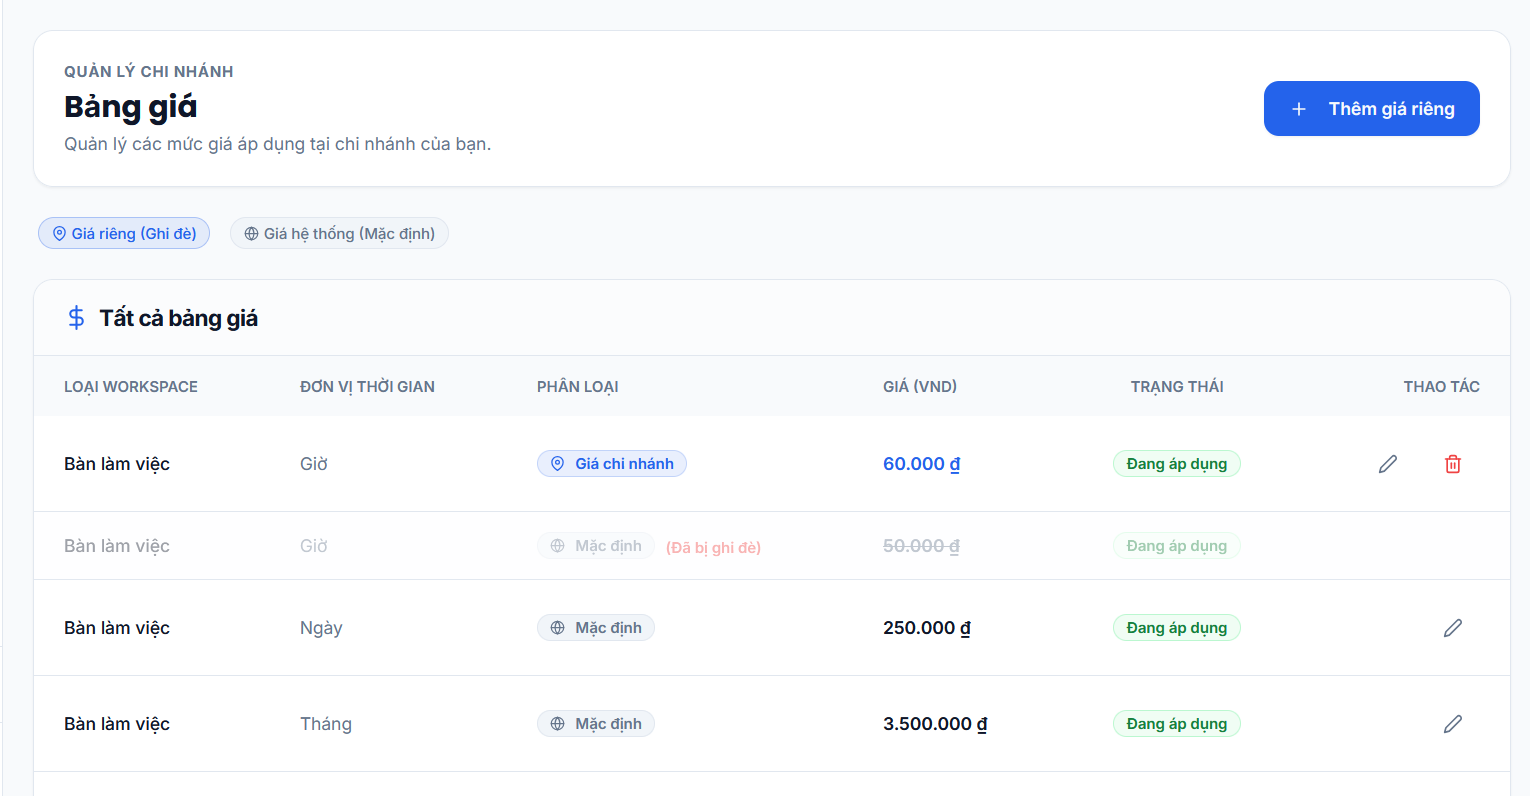
\includegraphics[width=0.9\textwidth]{Images/Chuong4/ui_ba_pricing_page.png}
    \caption{Giao diện thiết lập và quản lý các gói cước dịch vụ không gian}
    \label{fig:ui_ba_pricing_page}
\end{figure}

\FloatBarrier

Bên cạnh không gian cốt lõi, giao diện Quản lý dịch vụ hỗ trợ chi nhánh định nghĩa và kiểm soát các tiện ích mở rộng như dịch vụ in ấn, đồ uống hoặc thiết bị hội họp, giúp đa dạng hóa nguồn thu.

\begin{figure}[H]
    \centering
    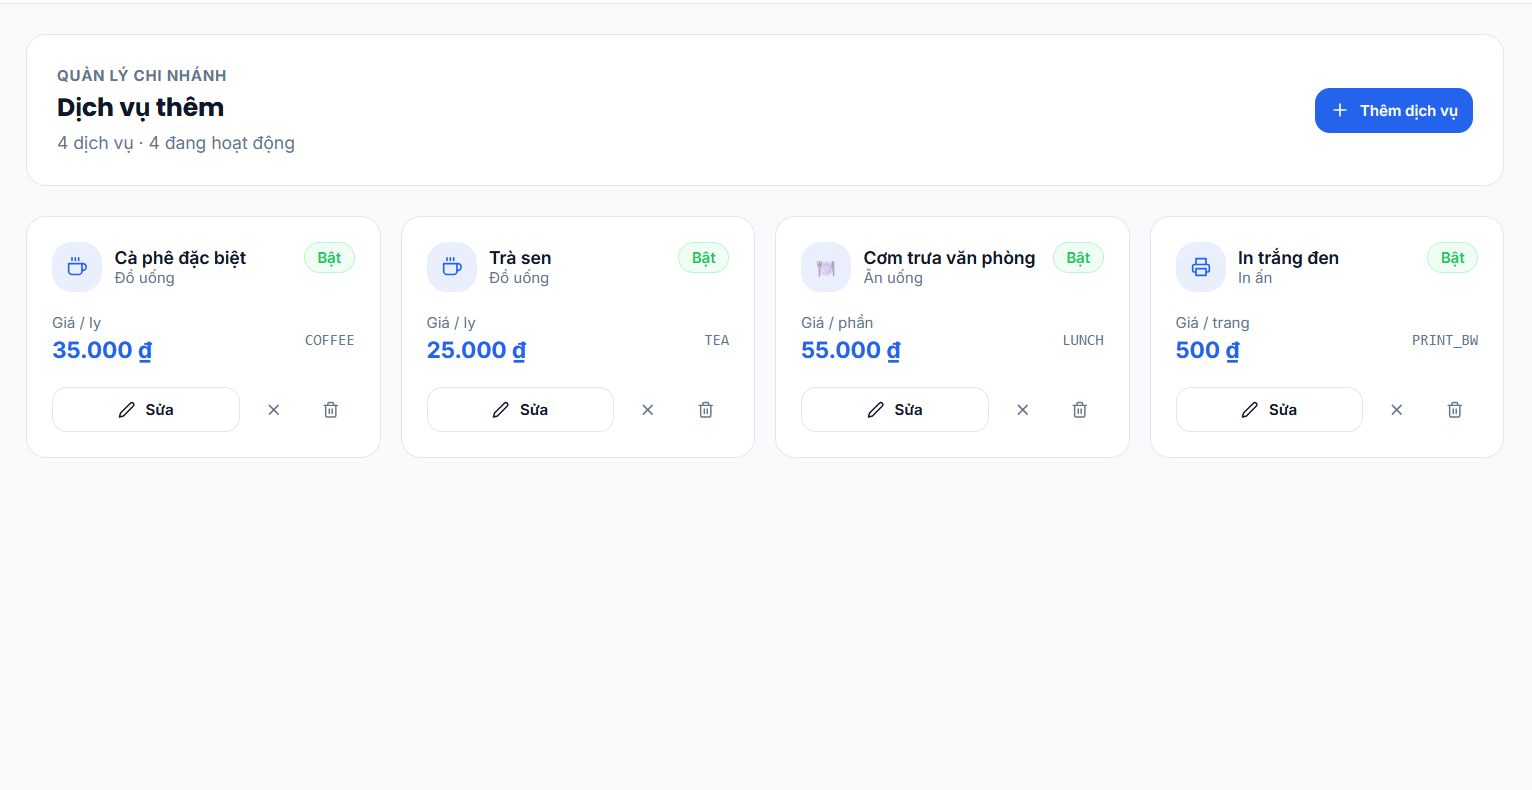
\includegraphics[width=0.9\textwidth]{Images/Chuong4/ui_ba_services_page.png}
    \caption{Giao diện quản lý danh mục các tiện ích và dịch vụ bổ sung}
    \label{fig:ui_ba_services_page}
\end{figure}

\FloatBarrier
\newpage

Giao diện Quản lý nhân sự tại chi nhánh hỗ trợ người quản lý trong việc phân ca, giám sát tiến độ công việc và đánh giá hiệu quả phục vụ của từng nhân viên thuộc quyền quản lý trực tiếp.

\begin{figure}[H]
    \centering
    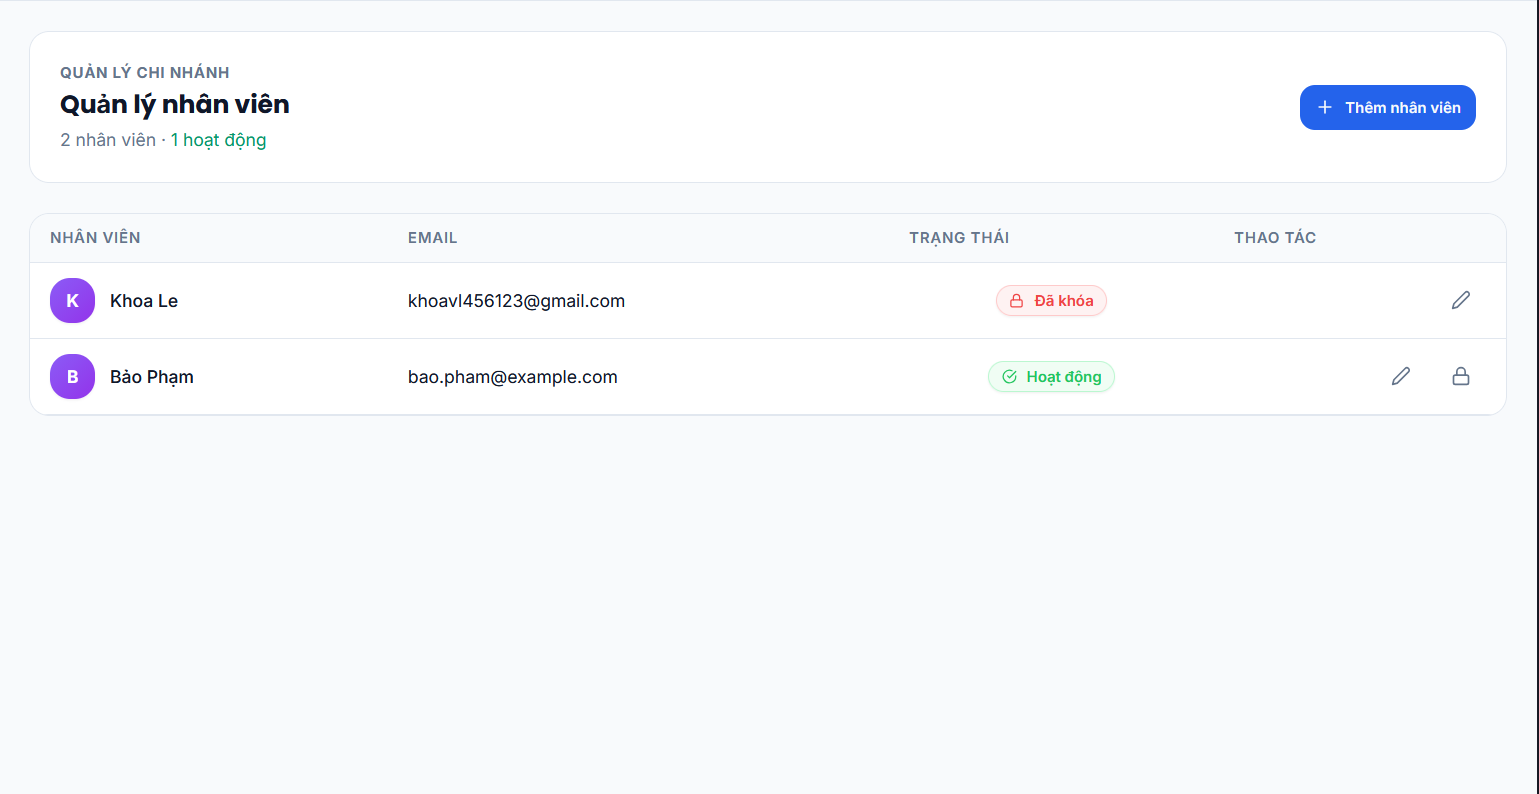
\includegraphics[width=0.9\textwidth]{Images/Chuong4/ui_ba_staff_page.png}
    \caption{Giao diện theo dõi danh sách và hoạt động của nhân viên cơ sở}
    \label{fig:ui_ba_staff_page}
\end{figure}

\FloatBarrier

Giao diện Báo cáo chi nhánh tập hợp các biểu đồ phân tích trực quan về hiệu suất tài chính, tỷ lệ lấp đầy trung bình và xu hướng sử dụng dịch vụ, làm cơ sở cho các quyết định điều hành ngắn và trung hạn. Ngoài ra trang còn cung cấp lịch sử hoạt động của chi nhánh.

\begin{figure}[H]
    \centering
    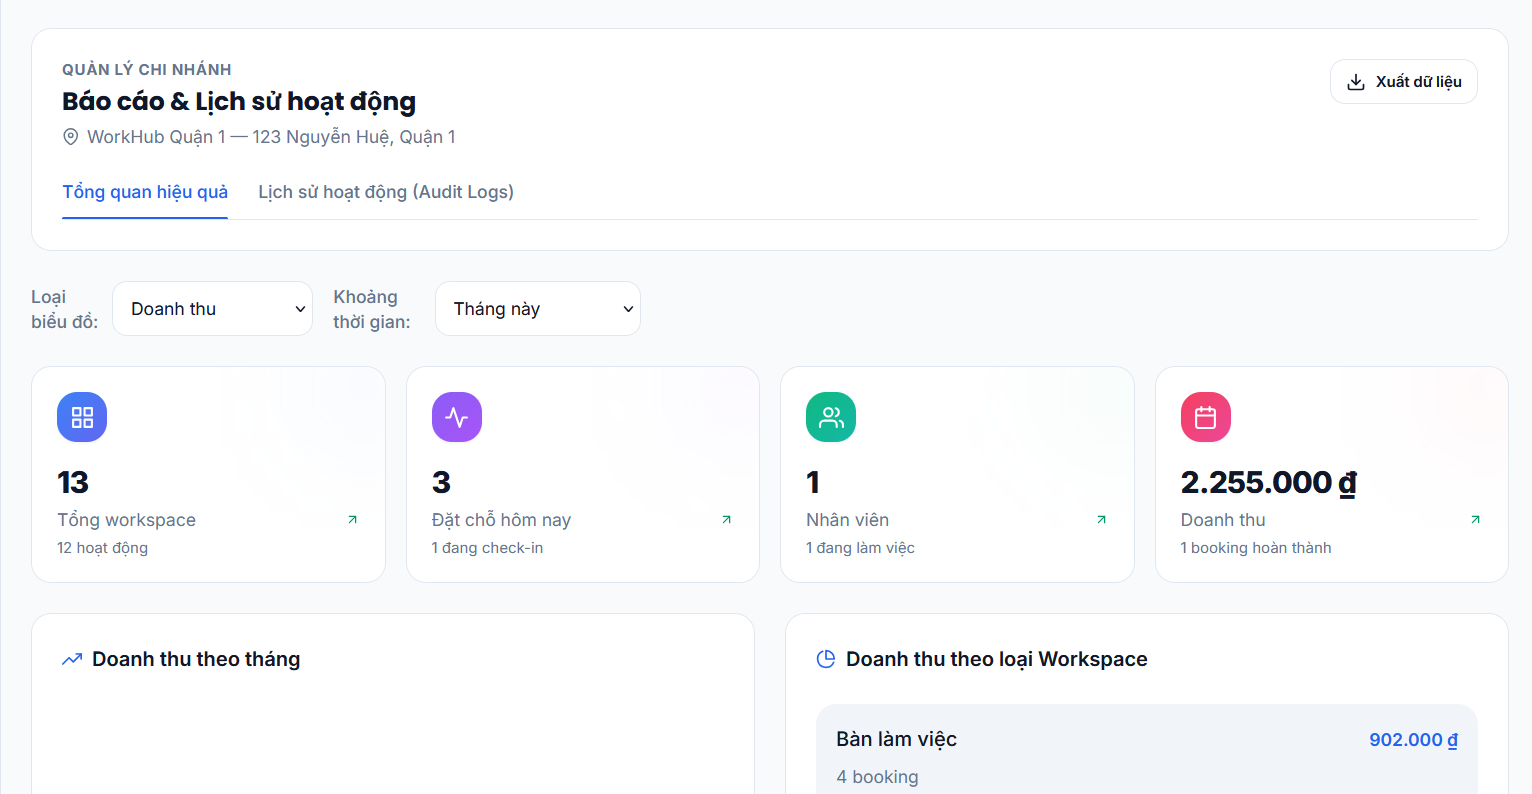
\includegraphics[width=0.9\textwidth]{Images/Chuong4/ui_ba_reports_page.png}
    \caption{Giao diện biểu đồ hóa dữ liệu kinh doanh và hiệu năng vận hành cục bộ}
    \label{fig:ui_ba_reports_page}
\end{figure}

\FloatBarrier
\newpage

\subsubsection{Phân hệ Giao diện Quản trị viên hệ thống (Admin)}

Phân hệ quản trị viên nắm giữ vai trò cao nhất, chịu trách nhiệm thiết lập các quy chuẩn chung, kiểm soát quy mô mạng lưới và giám sát tính bảo mật của toàn bộ nền tảng.

Giao diện Quản lý mạng lưới chi nhánh cho phép quản trị viên xem xét quy mô tổng thể, cấu hình thông tin định danh mới hoặc tạm ngưng các cơ sở không còn hoạt động.

\begin{figure}[H]
    \centering
    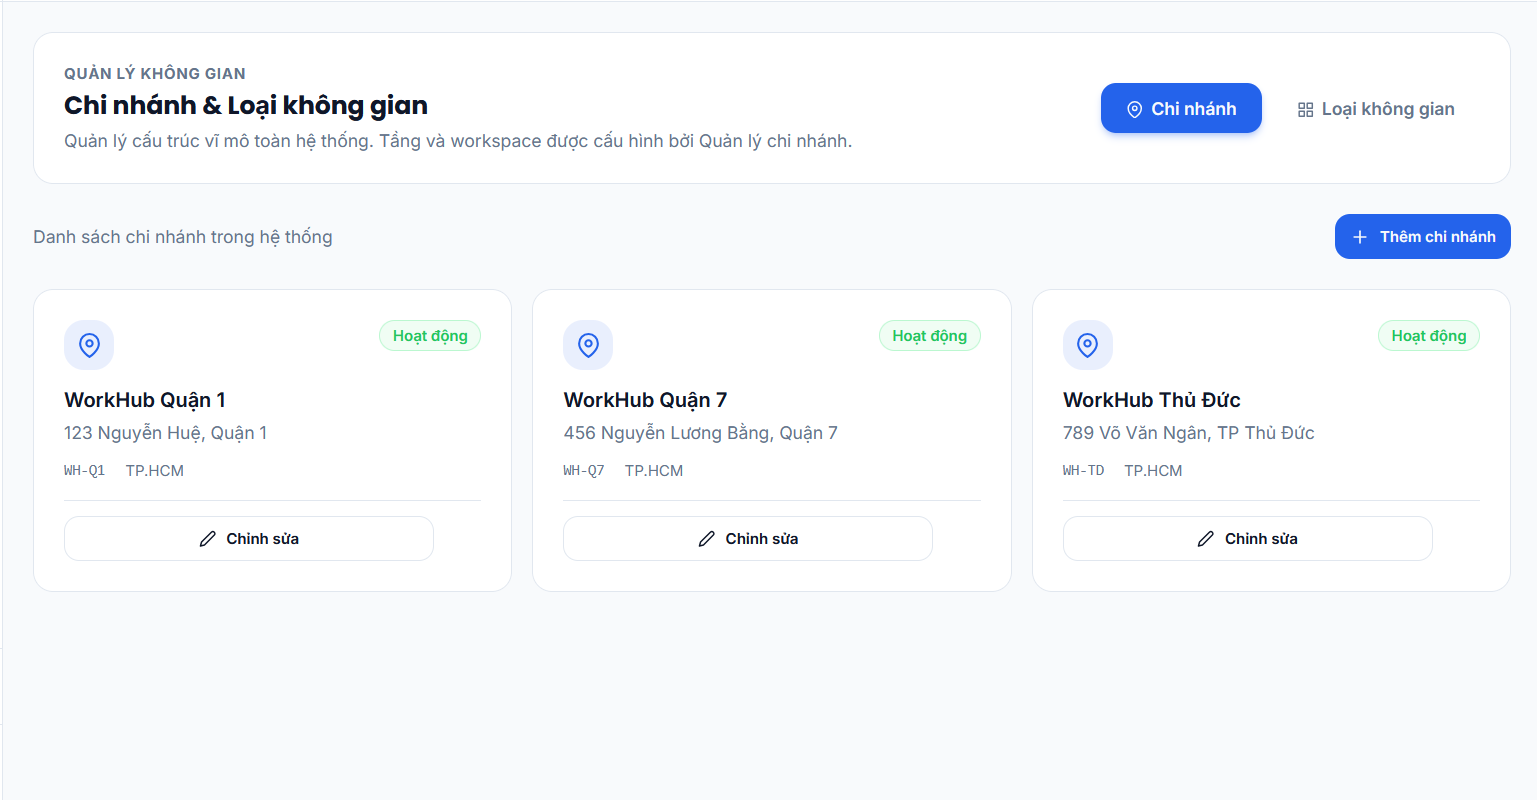
\includegraphics[width=0.9\textwidth]{Images/Chuong4/ui_admin_branches_page.png}
    \caption{Giao diện điều phối toàn cục danh sách các cơ sở thuộc hệ thống}
    \label{fig:ui_admin_branches_page}
\end{figure}

\FloatBarrier

Giao diện Quản lý tài khoản là trung tâm phân quyền và bảo mật. Quản trị viên sử dụng công cụ này để kiểm soát vai trò, gán chức vụ cho nhân sự và khóa các tài khoản vi phạm chính sách nền tảng.

\begin{figure}[H]
    \centering
    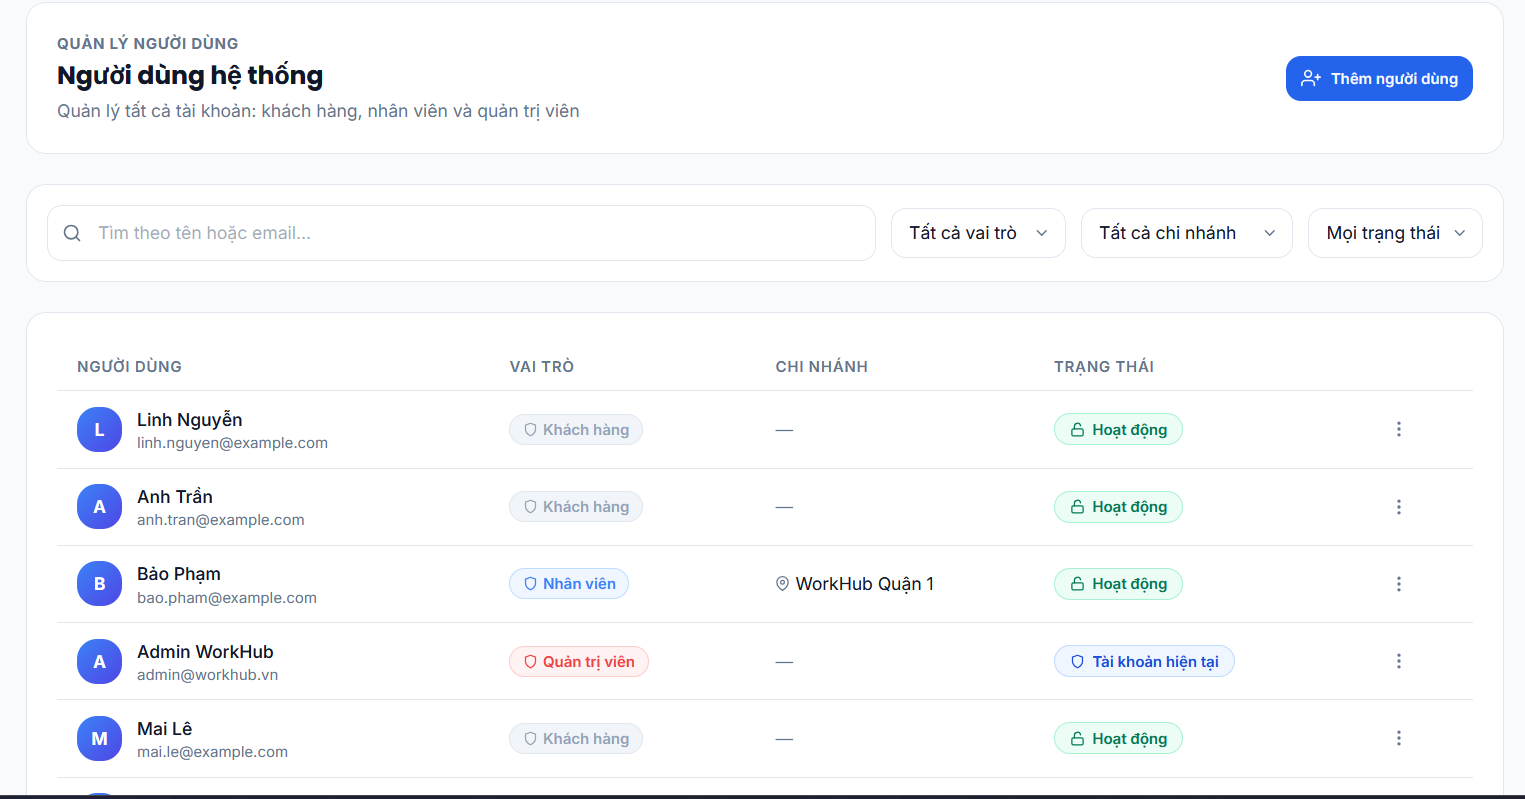
\includegraphics[width=0.9\textwidth]{Images/Chuong4/ui_admin_users_page.png}
    \caption{Giao diện kiểm soát thông tin, phân quyền và trạng thái tài khoản}
    \label{fig:ui_admin_users_page}
\end{figure}

\FloatBarrier
\newpage

Giao diện Quản lý chính sách hủy thiết lập các quy tắc cốt lõi về việc hoàn tiền và phí phạt. Chức năng này giúp hệ thống tự động hóa quá trình xử lý rủi ro khi khách hàng thay đổi lịch trình đột xuất.

\begin{figure}[H]
    \centering
    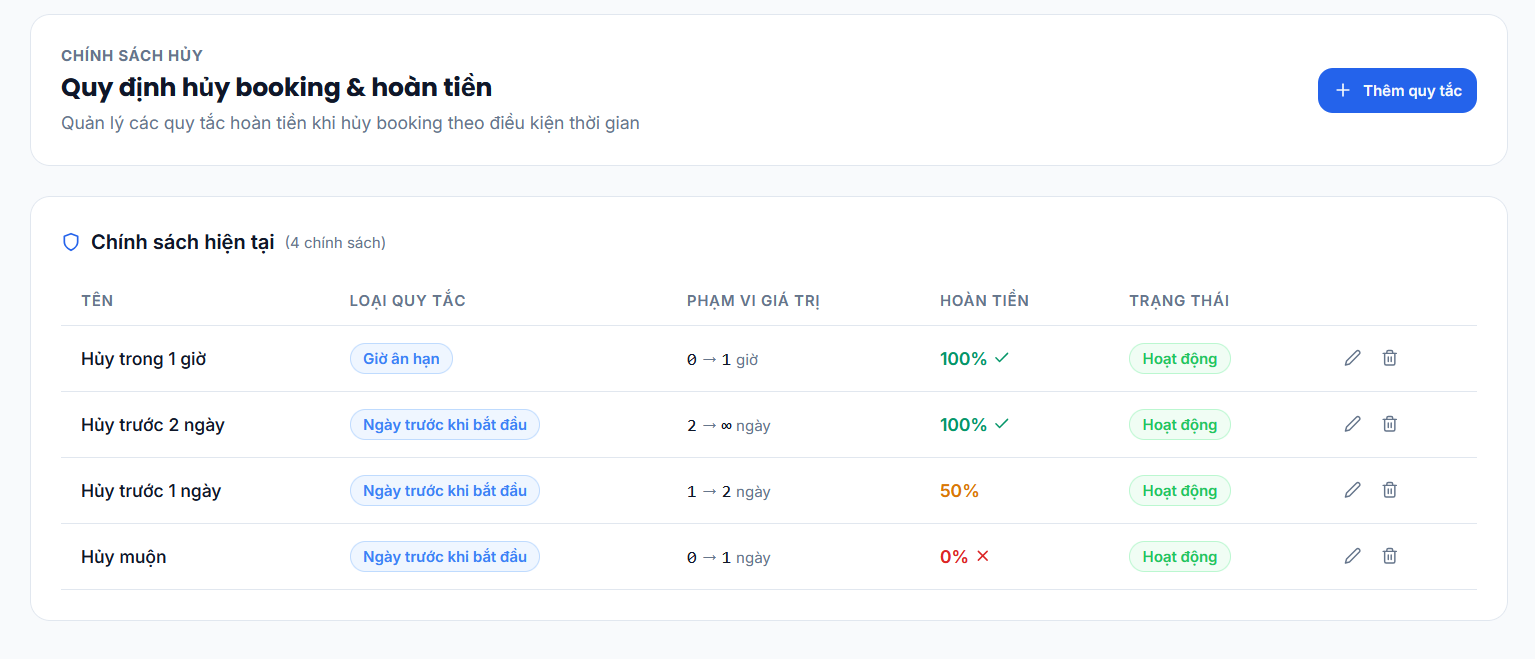
\includegraphics[width=0.9\textwidth]{Images/Chuong4/ui_admin_cancellation_page.png}
    \caption{Giao diện thiết lập khung pháp lý điện tử và các quy tắc hoàn tiền}
    \label{fig:ui_admin_cancellation_page}
\end{figure}

\FloatBarrier

Tương tự như cấu hình cục bộ, giao diện Quản lý dịch vụ tổng quy định danh mục gốc cho các tiện ích bổ sung, đảm bảo tính đồng bộ về mặt định dạng và tiêu chuẩn dịch vụ trên toàn chuỗi.

\begin{figure}[H]
    \centering
    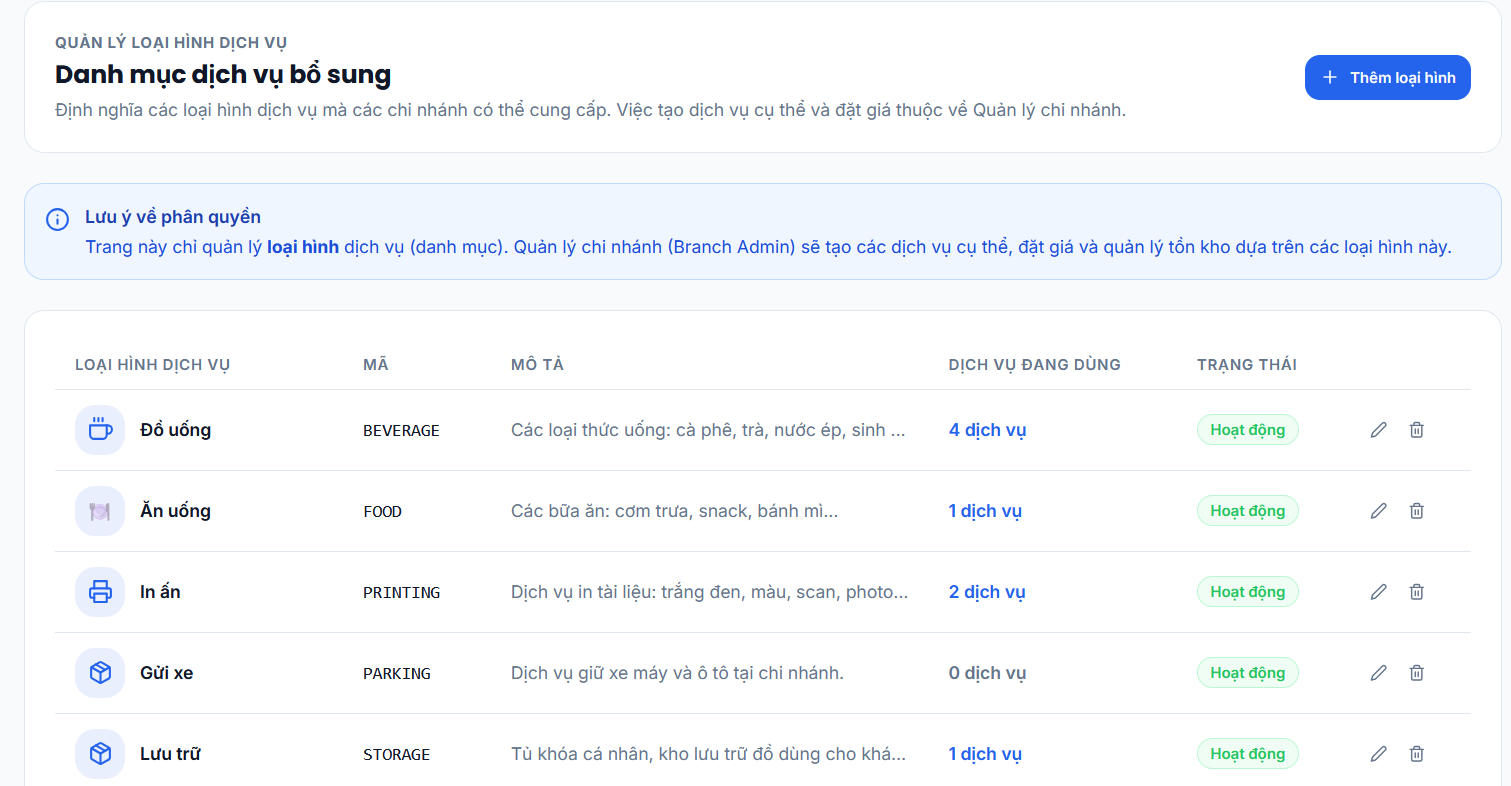
\includegraphics[width=0.9\textwidth]{Images/Chuong4/ui_admin_extra_services_page.png}
    \caption{Giao diện chuẩn hóa danh sách các dịch vụ tiện ích trên toàn nền tảng}
    \label{fig:ui_admin_extra_services_page}
\end{figure}

\FloatBarrier
\newpage

Giao diện Tra cứu nhật ký hệ thống (Audit Log) lưu trữ toàn vẹn lịch sử các tác động lên cơ sở dữ liệu. Đây là công cụ đắc lực phục vụ cho việc kiểm toán, truy vết nguồn gốc thay đổi và phát hiện các rủi ro nội bộ.

\begin{figure}[H]
    \centering
    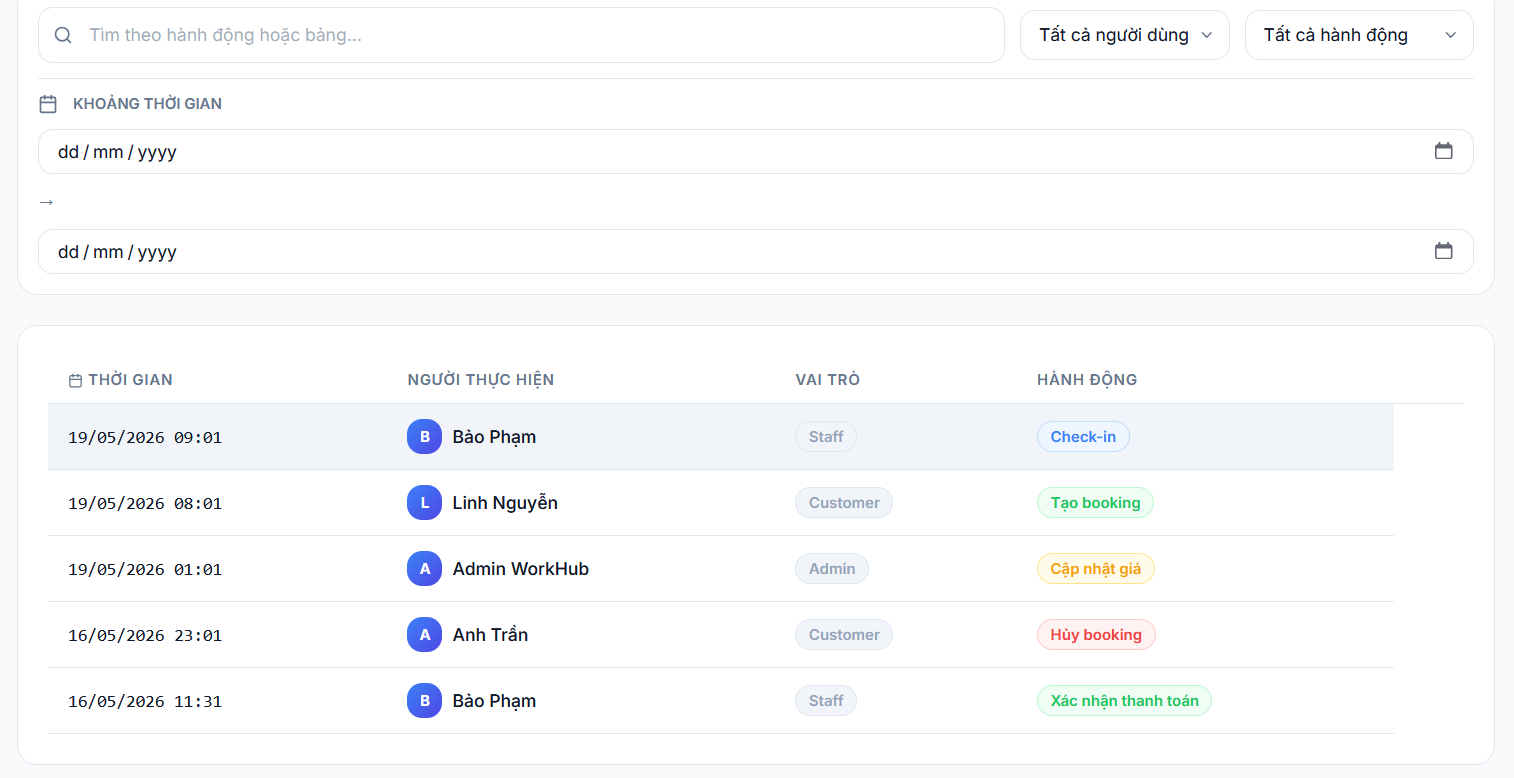
\includegraphics[width=0.9\textwidth]{Images/Chuong4/ui_admin_audit_log_page.png}
    \caption{Giao diện theo dõi vết thao tác dữ liệu nhằm đảm bảo tính minh bạch}
    \label{fig:ui_admin_audit_log_page}
\end{figure}

\FloatBarrier

Cuối cùng, giao diện Báo cáo tổng quan hệ thống đóng vai trò như một trạm chỉ huy chiến lược. Nơi này tổng hợp luồng dữ liệu từ tất cả chi nhánh, cung cấp các phân tích dự báo và số liệu vĩ mô hỗ trợ ban lãnh đạo ra quyết định.

\begin{figure}[H]
    \centering
    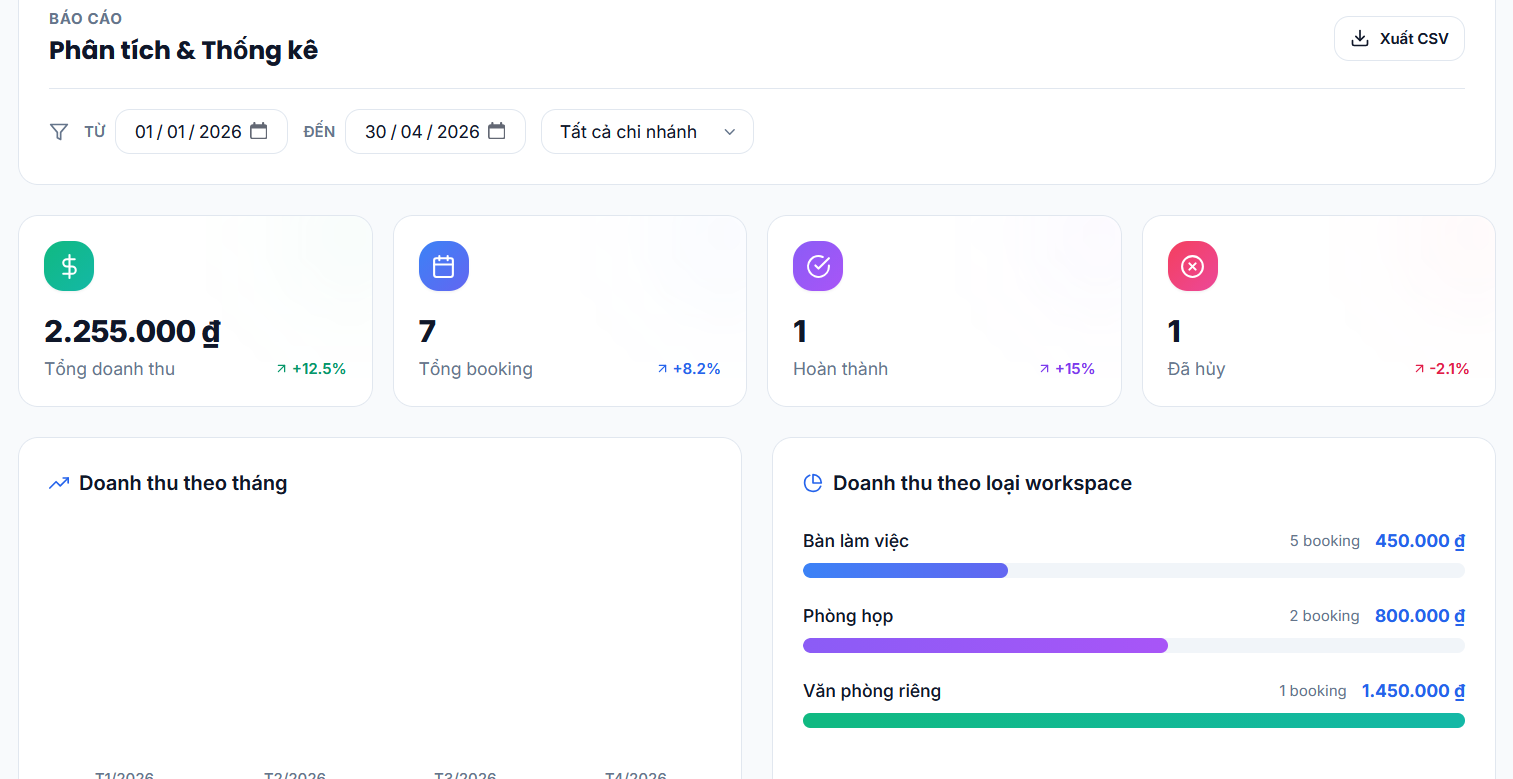
\includegraphics[width=0.9\textwidth]{Images/Chuong4/ui_admin_reports_page.png}
    \caption{Giao diện phân tích chuyên sâu về hiệu quả kinh doanh của toàn bộ hệ thống}
    \label{fig:ui_admin_reports_page}
\end{figure}

\FloatBarrier